%\documentclass[preprint,12pt]{elsarticle}

%% Use the option review to obtain double line spacing
%% \documentclass[authoryear,preprint,review,12pt]{elsarticle}

%% Use the options 1p,twocolumn; 3p; 3p,twocolumn; 5p; or 5p,twocolumn
%% for a journal layout:
 \documentclass[final,1p,times]{elsarticle}
%% \documentclass[final,1p,times,twocolumn]{elsarticle}
%% \documentclass[final,3p,times]{elsarticle}
%% \documentclass[final,3p,times,twocolumn]{elsarticle}
%% \documentclass[final,5p,times]{elsarticle}
%% \documentclass[final,5p,times,twocolumn]{elsarticle}

%% For including figures, graphicx.sty has been loaded in
%% elsarticle.cls. If you prefer to use the old commands
\usepackage{epsfig}

%% The amssymb package provides various useful mathematical symbols
\usepackage{amssymb}
%% The amsthm package provides extended theorem environments
\usepackage{amsthm}

\usepackage{amsmath}

\usepackage{CJK}
\usepackage{color}

\usepackage{enumitem}
\usepackage{rotating}

%% The lineno packages adds line numbers. Start line numbering with
%% \begin{linenumbers}, end it with \end{linenumbers}. Or switch it on
%% for the whole article with \linenumbers.
%% \usepackage{lineno}

%\journal{Nuclear Physics B}

\hyphenation{data-log}

\begin{document}

\newtheorem{theorem}{Theorem}
\newtheorem{definition}{Definition}
\newtheorem{example}{Example}
\newtheorem{lemma}{Lemma}
\newtheorem{corollary}{Corollary}

\begin{frontmatter}

%% Title, authors and addresses

%% use the tnoteref command within \title for footnotes;
%% use the tnotetext command for theassociated footnote;
%% use the fnref command within \author or \address for footnotes;
%% use the fntext command for theassociated footnote;
%% use the corref command within \author for corresponding author footnotes;
%% use the cortext command for theassociated footnote;
%% use the ead command for the email address,
%% and the form \ead[url] for the home page:
%% \title{Title\tnoteref{label1}}
%% \tnotetext[label1]{}
%% \author{Name\corref{cor1}\fnref{label2}}
%% \ead{email address}
%% \ead[url]{home page}
%% \fntext[label2]{}
%% \cortext[cor1]{}
%% \address{Address\fnref{label3}}
%% \fntext[label3]{}

\title{Parallel Tractability of Ontology\\
Materialization: Technique and Practice}

%% use optional labels to link authors explicitly to addresses:
%% \author[label1,label2]{}
%% \address[label1]{}
%% \address[label2]{}

\author[add1]{Zhangquan Zhou \corref{cor1}}
\ead{quanzz1129@gmail.com}
\cortext[cor1]{Corresponding author}

\author[add1]{Guilin Qi}
\ead{gqi@seu.edu.cn}

\author[add2]{Birte Glimm}
\ead{birte.glimm@uni-ulm.de}

\address[add1]{
    School of Computer Science, Southeast University, China
}

\address[add2]{
    Institute of Artificial Intelligence, University of Ulm
}

\begin{abstract}
  Materialization is an important reasoning service for many
  ontology-based applications, but the rapid growth of semantic data
  poses the challenge to efficiently perform materialization on
  large-scale ontologies. Parallel materialization algorithms work
  well for some ontologies, which is not always explained by the
  theoretical results. For example, for the YAGO ontology
  parallelization works well, although the reasoning problem for the
  used ontology language is not in \texttt{NC}, i.e., the theoretical
  complexity class for \emph{parallel tractability}. This motivates us
  to study the problem of \emph{parallel tractability} of ontology
  materialization from a theoretical perspective. We focus on the
  datalog rewritable ontology languages DL-Lite and Description Horn
  Logic (DHL) and propose algorithms, called \texttt{NC} algorithms,
  to identify classes of ontologies for which materialization is
  tractable in parallel. To verify the practical usability of the
  above results, we analyze real-world datasets and show that for many
  ontologies expressed in DHL materialization is tractable in
  parallel. The implementation of our optimized parallel algorithm
  shows performance improvements over the highly optimized
  state-of-the-art reasoner RDFox on ontologies for which
  materialization is tractable in parallel.
\end{abstract}

\begin{keyword}
ontology \sep materialization \sep datalog \sep parallel tractability \sep NC complexity
\end{keyword}

\end{frontmatter}

%% \linenumbers


\section{Introduction}
\label{sec:introduction}

The Web Ontology Language (OWL)\footnote{The latest version is OWL 2: http://www.w3.org/TR/owl2-overview/}
is an important standard for ontology languages in the Semantic Web and knowledge-based applications.
In many of these applications, \emph{materialization} plays an important role, which is the reasoning task of computing all implicit
\emph{facts} that follow from a given ontology \cite{handbook}. Ontology developers and users employ materialization to optimize tasks such as query answering, ontology diagnosis or debugging. Since large amounts of semantic data
are being generated at an increasing pace by sensor networks, government authorities and social
media \cite{LehmbergRMB16,MeuselBP15}, it is challenging to conduct materialization on such large-scale ontologies efficiently.

For the ontology language RDFS and its extended fragments, approaches for parallel reasoning and for employing parallel computing platforms exist
 \cite{MotikNPHO14,PetersSZ15,SubercazeGCL16}. Several optimization strategies, e.g., dictionary encoding, balancing workload
and data partitioning, are further studied to enhance parallel RDFS reasoning. There are also parallel implementations for scalable
reasoning over ontologies that use highly expressive ontology languages \cite{SteigmillerLG14,WuH12}. The different approaches utilize different kinds of computing platforms to make reasoning tasks more efficient in parallel, e.g., supercomputers \cite{Hoeksema2011,GoodmanJMAAH11},
MapReduce \cite{UrbaniKMHB12} and GPU servers \cite{HeinoP12}.

The effectiveness of parallel reasoning for the above mentioned techniques is empirically verified on different test datasets.
However, materialization is not tractable in parallel for most of the popular ontology languages with \texttt{PTime}-complete or higher complexity \cite{Raymond95}. In particular, this is the case for RDFS and datalog rewritable ontology languages and, therefore, the efficiency of reasoning may not be
improved using a parallel implementation. A possible reason for the apparent high performance of parallel
reasoning is that the utilized test datasets do not fall into the worst cases in terms of computational complexity. Also some well-known, large-scale ontologies such as YAGO show good performance for parallel
reasoning \cite{KolovskiWE10}, although they are expressed in ontology languages that are, in theory, not tractable in parallel.
On the other hand, there are ontologies for which materialization performance does not improve by parallelism and our experiments in Section~\ref{sec:evaluation} confirm this.
The current theoretical work of parallel ontology reasoning can hardly explain this.
While one can try out different parallel implementations to see whether an ontology can be handled by (one of) them efficiently,
we study the problem of parallel tractability in theory and identify properties that make an ontology tractable in parallel.
These properties can further be used to optimize parallel algorithms and to guide ontology engineers in creating ontologies
for which parallel tractability can be guaranteed theoretically.

According to \citet{MotikNPHO14}, many real large-scale ontologies are essentially expressed in ontology languages
that can be rewritten into datalog rules. We follow this argumentation and focus on such datalog rewritable ontology languages in this paper.
The main target of this paper is to identify classes of datalog rewritable ontologies such that materialization
over these ontologies is tractable in parallel, i.e., falls into the parallel complexity class \texttt{NC} \cite{Raymond95}.
This complexity class consists of problems that can be solved efficiently in parallel.
To show that a problem is in \texttt{NC}, one can give an \emph{\texttt{NC} algorithm} that handles this problem
using parallel computation \cite{Raymond95}.
An \texttt{NC} algorithm is required to terminate in parallel poly-logarithmic time.
However, \mbox{current} materialization algorithms of datalog rewritable ontology languages
(e.g., the core algorithm used in RDFox \cite{MotikNPHO14}) are not \texttt{NC} algorithms
since they are designed for general datalog programs and have \texttt{PTime}-complete complexity.
Thus, we first give \texttt{NC} algorithms that perform materialization
and then identify the corresponding classes of datalog rewritable ontologies (called \emph{parallel tractability classes})
that can be handled by these \texttt{NC} algorithms. To make the proposed \texttt{NC} algorithms practical,
we also discuss how to optimize and implement them.

In the practical part of this work, we study specific datalog rewritable ontology languages.
We first focus on the ontology language DL-Lite \cite{CalvaneseGLLR07} to clarify how to apply the above \texttt{NC} algorithms
to study parallel tractability of ontology materialization.
We show that DL-Lite$_{\text{core}}$ and DL-Lite$_\mathcal{R}$ are tractable in parallel.
We then study the ontology language Description Horn Logic (DHL) \cite{GrosofHVD03}, which is the intersection of datalog and OWL
in terms of expressivity. We give a case of a DHL ontology where materialization can hardly be parallelized.
Based on the analysis of this case, we propose to restrict the usage of DHL such that materialization over the
restricted ontologies can be handled by the proposed \texttt{NC} algorithms.
We further extend the results to an extension of DHL that also allows complex role inclusion axioms.
Finally, we analyze the well-known benchmark, LUBM, and the real-world dataset, YAGO, and
show that these ontologies satisfy the
proposed restrictions and, hence, belong to the parallel tractability classes.
We implement a system based on an optimized \texttt{NC} algorithm for DHL materialization,
which we compare to the state-of-the-art reasoner RDFox \cite{MotikNPHO14}.
The experimental results show that the optimizations proposed in this paper result in a
better performance on ontologies that are
tractable in parallel compared to RDFox.

The remainder of the paper is organized as follows. In Section~\ref{sec:background}, we introduce some basic notions.
We then give two \texttt{NC} algorithms for ontology materialization in Section~\ref{sec:ptclass}.
We study parallel tractability of materialization in DL-Lite, DHL and an extension of DHL in Section~\ref{sec:ptonto}.
In Section~\ref{sec:practicalAlg},
we discuss how to optimize and implement the given \texttt{NC} algorithms.
We analyze the LUBM and the YAGO ontologies and evaluate our implementation in Section~\ref{sec:evaluation}.
Finally, we discuss related work in Section~\ref{sec:related} and conclude in Section~\ref{sec:conclusion}. Detailed proofs of the theorems and lemmas in this paper are given in the appendix.



%%% Local Variables:
%%% mode: latex
%%% TeX-master: "parallel-tractability-J"
%%% End:


\section{Background Knowledge}
\label{sec:background}

In this section, we introduce some basic notions that are needed to introduce our approach.


\subsection{Datalog}

We discuss the main issues in this paper using standard datalog notions.
In datalog \cite{database}, a \emph{term} is a variable or a constant. An \emph{atom} $A$
is defined by $A\equiv p(t_1,...,t_n)$ where $p$ is a \emph{predicate} (or \emph{relational})
name, $t_1,...,t_n$ are terms, and $n$ is the arity of $p$. If all the terms in an atom $A$ are
constants, then $A$ is called a \emph{ground atom}.
A datalog \emph{rule} is of the form: `$B_1,...,B_n\rightarrow H$',\footnote{In datalog rules, a comma
represents a Boolean conjunction `$\wedge$'.} where $H$ is referred to as
the \emph{head atom} and $B_1,...,B_n$ the \emph{body atoms}. Each variable in the head atom
of a rule must occur in at least one body atom of the same rule. A \emph{fact} is a rule of
the form `$\rightarrow H$', i.e., a rule with an empty body and the head $H$ being a ground atom.
A datalog program $P$ consists of rules and facts.
A \emph{substitution} $\theta$ is a partial mapping of variables to constants.
For an atom $A$, $A\theta$ is the result of replacing each variable $x$ in $A$
with $\theta(x)$ if the latter is defined. We call $\theta$ a \emph{ground substitution}
if each defined $A\theta$ is a ground atom.
A \emph{ground instantiation} of a rule is obtained by applying a ground substitution on all
the terms in this rule with respect to a finite set of constants occurring in $P$.
Furthermore the ground instantiation of $P$, denoted by $P^*$,
consists of all ground instantiations of rules in $P$.
The predicates occurring only in the body  of some rules are called \emph{EDB predicates},
while the predicates that may occur as head atoms are called \emph{IDB predicates}.


\subsection{DHL and DL-Lite}

In what follows, we use $\textbf{CN}$, $\textbf{RN}$ and $\textbf{IN}$
to denote three disjoint countably
infinite sets of \emph{concept names, role names}, and \emph{individual names} respectively.
The set of roles is defined as $\textbf{R}:=\textbf{RN}\cup\{R^-|R\in\textbf{RN}\}$
where $R^-$ is the \emph{inverse role} of $R$.
For ease of discussion, we focus on the \emph{simple forms} of axioms shown
in the left column of Table~1. These simple forms can be obtained by using
well-known \emph{structure transformation} techniques \cite{KrotzschRH07,Kazakov09}.

DHL (short for \emph{description horn logic}) \cite{GrosofHVD03} is introduced as an
intersection of description logic (DL) and datalog in terms of expressivity.
We define a DHL ontology $\mathcal{O}$ as a triple:
$\mathcal{O}=\langle\mathcal{T},\mathcal{R},\mathcal{A}\rangle$, where
$\mathcal{T}$ denotes the TBox containing axioms of the forms (T1-T3);
$\mathcal{R}$ is the RBox that is a set of axioms of the forms (R1-R3);
$\mathcal{A}$ is the ABox containing \emph{assertions} of the forms (A1) and (A2).
In an axiom of either of  the forms (T1-T3 and R1-R3), concepts $A_{(i)}$ and $B$ are either
concept names, \emph{top concept} ($\top$) or \emph{bottom concept} ($\bot$); $R$ and $S_{(i)}$
are roles in $\textbf{R}$.
For an axiom of the form $A\sqsubseteq\forall R.B$ that is also allowed in DHL, we only consider its
equivalent form $\exists R^-.A\sqsubseteq B$.

DHL is related with other ontology languages.
First, DHL is essentially a fragment of the description logic Horn-$\mathcal{SHOIQ}$ with
disallowing \emph{nominal}, \emph{number restriction} and
right-hand \emph{existential restriction} ($A\sqsubseteq\exists R.B$).
Second, the expressivity of DHL covers that of RDFS to some extent \cite{GrosofHVD03}.
Reasoning with RDFS ontologies is \texttt{NP}-complete \cite{Horst05}
and, thus, is not parallelly tractable.
However, by applying some simplifications and restrictions, RDFS ontologies can be
expressed in DHL \cite{GrosofHVD03} that has \texttt{PTime}-complete complexity for
materialization.

\begin{table}
\begin{center}
\begin{tabular}{lcc}
\multicolumn{3}{c}{\textbf{Table 1: Axioms and corresponding datalog rules}}\\
\hline
&~~~~~~~~~~~~~~~~~~~~~~~~Axioms~~~~~~~~~~~~~~~~~~~~~~~~&~~~~~~~~~~~~~~~~~~~~~~~~Datalog Rules~~~~~~~~~~~~~~~~~~~~~~~~\\
\hline
\hline
(T1)& $A\sqsubseteq B$& $A(x)\rightarrow B(x)$\\
(T2)& $A_1\sqcap A_2\sqsubseteq B$& $A_1(x), A_2(x)\rightarrow B(x)$\\
(T3)& $\exists R.A\sqsubseteq B$& $R(x,y), A(y)\rightarrow B(x)$\\
(T4)& $A\sqsubseteq\exists R$& $A(x)\rightarrow R(x, o_{R}^A)$\\

\hline
(R1)& $S\sqsubseteq R$& $S(x,y)\rightarrow R(x,y)$\\
(R2)& $S\sqsubseteq R^-$& $S(x,y)\rightarrow R(y,x)$\\
(R3)& $R\circ R\sqsubseteq R$& $R(x,y), R(y,z)\rightarrow R(x,z)$\\
(R4)& $R_1\circ R_2\sqsubseteq R$&$R_1(x,y),R_2(y,z)\rightarrow R(x,z)$\\

\hline
(A1)& $A(a)$& $A(a)$\\
(A2)& $R(a,b)$& $R(a,b)$\\
\hline
\end{tabular}
\label{tab:dhl}
\end{center}
\end{table}

In the initial work of DHL \cite{GrosofHVD03}, \emph{complex role inclusion axioms} (complex RIAs) of
the form $R_1\circ...\circ R_n\sqsubseteq R$ are not considered, although they can be
naturally transformed to datalog rules.
In this paper, we also consider an extension of DHL (denoted by DHL($\circ$))
that allows complex RIAs. Since a complex RIA can be transformed to
several axioms of the form (R4), we then require that an
RBox $\mathcal{R}$ of a DHL($\circ$) ontology can contain
axioms of the forms (R1-R4). Note that (R3) is actually a special
case of (R4).

DL-Lite is a group of ontology languages designed for highly-efficient
query answering through knowledge
and underpins the OWL profile OWL QL \cite{CalvaneseGLLR07}.
DL-Lite$_{core}$ and DL-Lite$_{\mathcal{R}}$ are the two basic fragments
in DL-Lite.
DL-Lite$_{core}$ requires that an TBox contains axioms of the forms (T1) $A\sqsubseteq B$,
(T2) $A_1\sqcap A_2\sqsubseteq B$ where $B\equiv\bot$, (T3) $\exists R.A\sqsubseteq B$
where $A\equiv\top$ or $B\equiv\bot$, and (T4) $A\sqsubseteq\exists R$,
an ABox contains \emph{assertions} of the forms (A1) and (A2), and
RBox is not involved. DL-Lite$_{\mathcal{R}}$ is an extension of DL-Lite$_{core}$,
which allows involving RBoxes that contain axioms of the forms (R1-R2).
If not specially specified, \emph{a DL-Lite ontology denotes a DL-Lite$_{\mathcal{R}}$ ontology
in the following paragraphs}.


\subsection{Ontology Materialization via Datalog Programs}

An ontology
expressed in DHL, DHL($\circ$), DL-Lite$_{core}$ or DL-Lite$_{\mathcal{R}}$ can be transformed to a datalog program
(see the corresponding rules in the right column of Table~1).
Note that, for an axiom of the form (T4) $A\sqsubseteq\exists R$, it should be transformed to
a first-order logic rule `$A(x)\rightarrow \exists y(R(x,y))$' where $y$ is called a \emph{free variable} (it is
not occurring in the head atom $A(x)$).
In this work, such a free variable $y$ is eliminated via Skolemisation into a new individual $o_{R}^A$
that corresponds to concept $A$ and role $R$. One can check that the elimination of free variables
does not influence the results of materialization by according to \cite{CalvaneseGLLR07}.

In what follows, for an ontology $\mathcal{O}=\langle\mathcal{T},\mathcal{R},\mathcal{A}\rangle$,
we also use $P=\langle R, \textbf{I}\rangle$ to represent the corresponding datalog program
where $R$ is the set of rules transformed from the axioms in $\mathcal{T}$ and $\mathcal{R}$,
$\textbf{I}$ is the set of facts that are directly copied from the assertions in $\mathcal{A}$.
Further, we use $R_1\sqsubseteq_{*}R_2$ to denote the smallest transitive reflexive relation
between roles such that $R_1\sqsubseteq R_2\in\mathcal{R}$ implies $R_1\sqsubseteq_{*}R_2$
and $R_1^-\sqsubseteq_{*}R_2^-$. In this paper, we also use the
notion of \emph{simple role}, which is initially proposed to restrict the
usage of highly expressive ontology languages \cite{HorrocksS04}.
Specifically, a role $S\in\textbf{R}$ is \emph{simple} if, (1) it has no subrole (including $S$)
occurring on the right-hand side of axioms of the forms (R3) and (R4); (2) $S^-$ is simple.

Based on the above representations, ontology materialization
corresponds to the evaluation of datalog programs.
Specifically, given a datalog program $P=\langle R, \textbf{I}\rangle$,
let $T_R(\textbf{I})=\{H\theta|\forall B_1,...,B_n\rightarrow H\in R, B_i\theta\in\textbf{I} (1\leq i\leq n)\}$,
where $\theta$ is some substitution; further let $T_R^{0}(\textbf{I})=\textbf{I}$ and
 $T_R^{i}(\textbf{I})=T_R^{i-1}(\textbf{I})\cup T_R(T_R^{i-1}(\textbf{I}))$ for each $i>0$.
The smallest integer $n$ such that $T_R^{n}(\textbf{I})= T_R^{n+1}(\textbf{I})$ is called \emph{stage},
and \emph{materialization} refers to the computation of $T_R^{n}(\textbf{I})$ with respect to $R$ and \textbf{I}.
$T_R^{n}(\textbf{I})$ is also called the \emph{fixpoint} and denoted by $T_R^{\omega}(\textbf{I})$.
We say that an atom $A$ is \emph{derivable} or can be \emph{derived} with respect
to the datalog program $P=\langle R, \textbf{I}\rangle$ if $A\in T_R^{\omega}(\textbf{I})$.
In this paper, we consider the data complexity of materialization, i.e., we \emph{assume that the rule set $R$ is fixed}
for any class of datalog programs.


\subsection{The NC Complexity}

The parallel complexity class NC, known as Nick$'$s
Class \cite{Raymond95}, is studied by theorists as a parallel complexity class
where each decision problem can be efficiently solved in parallel.
Specifically, a decision problem in the NC class
can be solved in poly-logarithmic time on a PRAM (parallel, random-access machine) with
a polynomial number of processors. We also say that an NC problem can be solved
in \emph{parallel poly-logarithmic time}.
Although the NC complexity is a theoretical analysis tool,
it has been shown that many NC problems can be solved efficiently in practice \cite{Raymond95}.

From the perspective of implementations, the NC problems are also highly
parallel feasible for other parallel models like BSP \cite{Valiant90}
and MapReduce \cite{KarloffSV10}. The NC complexity is originally defined
as a class of decision problems. Since we study the problem of materialization, we do not
require in this work that a problem should be a decision problem in NC.
In addition, since many parallel reasoning systems (see related work in Section~\ref{sec:related})
are implemented on shared-memory platforms, we
study all the issues in this work by assuming that the running machines are in
shared-memory configurations.



%%% Local Variables:
%%% mode: latex
%%% TeX-master: "parallel-tractability-J"
%%% End:


\section{Parallel Tractability of Datalog Programs}
\label{sec:ptclass}

Our target is to find for which kinds of ontologies (not ontology languages)
materialization is tractable in parallel. We consider data complexity,
i.e., we consider classes of datalog programs which share a fixed the rule set. 
The data complexity of the materialization problem in this case is
$\texttt{PTime}$-complete, which is considered to be inherently sequential in the worst
case \cite{Raymond95}.
% Since we assume that, for any class of datalog programs where the rule
% set of each datalog program is fixed, the materialization problem is, thus, in data complexity
% $\texttt{PTime}$-complete, which is considered to be inherently sequential in the worst
% case \cite{Raymond95}.
In other words, the materialization problem of 
datalog programs cannot be solved in parallel poly-logarithmic time unless \texttt{P}=\texttt{NC}.
Thus, we say that \emph{materialization for a class of datalog programs is tractable in parallel
if there exists an algorithm that handles this class of datalog programs and runs in parallel
poly-logarithmic time. Such an algorithm is also called an \texttt{NC} algorithm.}
In this section, we identify such classes of datalog programs by studying different \texttt{NC} algorithms.


\subsection{Parallel Tractability Classes}

We first give the following definition for a class of datalog programs
that is tractable in parallel, i.e., an \texttt{NC} algorithm exists for handling each datalog program in this class.

\begin{definition}\label{def:ptd}
\textbf{(Parallel Tractability Class)} Given a class $\mathcal{D}$ of
datalog programs sharing the same rule set, we say that $\mathcal{D}$
is a class of datalog program with \emph{p}arallel
\emph{t}ractability, short a \emph{\texttt{PTD} class}, 
if there exists an \texttt{NC} algorithm that performs sound and complete materialization for each datalog program
in $\mathcal{D}$. The corresponding class of ontologies of $\mathcal{D}$ is called a
class of ontologies with parallel tractability, short a \texttt{PTO} class.
\end{definition}

According to the above definition, if we find an \texttt{NC} algorithm $\mathsf{A}$
for datalog materialization, then we can identify a \texttt{PTD} class $\mathcal{D}_{\mathsf{A}}$,
which is the class of all datalog programs that can be handled by $\mathsf{A}$.
However, current materialization algorithms of datalog rewritable ontology languages
(e.g., the core algorithm used in RDFox \cite{MotikNPHO14}) are not \texttt{NC} algorithms
due to their \texttt{PTime}-complete complexity, since they are
designed for handling general datalog programs. Thus, we proceed to
devise specific \texttt{NC} algorithms.
In the following, we first give a parallel materialization algorithm that works for
general datalog programs. We then restrict this algorithm to an \texttt{NC} version
and identify the target \texttt{PTD} class.


\subsection{Materialization Graph}

In order to give a parallel materialization algorithm,
we introduce the notion of \emph{materialization graphs}, which
facilitates the analysis of the given algorithm.

\begin{definition}
\textbf{(Materialization Graph)}\label{def:mg}
A \emph{materialization graph}, with respect to
a datalog program $P=\langle R, \textbf{I}\rangle$, is a directed acyclic graph
denoted by $\mathcal{G}=\langle V, E\rangle$ where,
\begin{enumerate}[leftmargin=4ex,label=$\bullet$]
  \item $V$ is the node set and $V\subseteq T_R^{\omega}(\textbf{I})$;
  \item $E$ is the edge set and $E\subseteq T_R^{\omega}(\textbf{I})\times T_R^{\omega}(\textbf{I})$.
\end{enumerate}
For each edge of the form $e(v_1, v_2)$ where $v_1$ and $v_2$ are two nodes,
we say that the node $v_1$ is the parent (node) of $v_2$ and the node $v_2$ is the child (node)
of $v_1$. Further, $\forall H,B_1,...,B_n\in V$, $\mathcal{G}$ satisfies the following conditions:
\begin{enumerate}[leftmargin=4ex,label=$\bullet$]
  \item $H$ has a parent node or a child node;
  \item if $H$ has the in-degree of $0$, then $H$ is an original fact of $P$;
  \item $B_1,...,B_n\rightarrow H\in P^*$ is satisfied if $e(B_1, H),...,e(B_n, H)\in E$ and
  $B_1,...,B_n$ are \d{all} the parents of $H$.
\end{enumerate}
\end{definition}

For some derived atom $H$, there may exist several rule instantiations where $H$
occurs as a head atom.
This also means that $H$ can be derived in different ways.
The condition in the definition above results in only one way of deriving $H$ being
described by a materialization graph.
Suppose $\mathcal{G}$ is a materialization graph such that the nodes
with in-degree 0 are the
original facts in $\textbf{I}$.
The size of $\mathcal{G}$, denoted by $|\mathcal{G}|$, is the number of nodes in $\mathcal{G}$.
The depth of $\mathcal{G}$, denoted by \texttt{depth}($\mathcal{G}$), is the maximal length of a path
in $\mathcal{G}$.
We next give an example of a materialization graph.\\

\begin{example}\label{exp:mg}
Consider a DHL($\circ$) ontology $\mathcal{O}_{ex_1}$ where the TBox is
$\{\exists R.A\sqsubseteq A\}$, the RBox is $\{S\circ R\sqsubseteq R\}$ and
the ABox is $\{A(b),R(a_1,b),S(a_i,a_{i-1})\}$ for $2\leq i\leq k$ and
$k$ is an integer greater than $2$.
The corresponding datalog program of this ontology is $P_{ex_1}=\langle R, \textbf{I}\rangle$
where $\textbf{I}$ contains all the assertions in the ABox
and $R$ contains the two rules `$R(x,y),A(y)\rightarrow A(x)$'
and `$S(x,y),R(y,z)\rightarrow R(x,z)$'.
The graph in Figure~\ref{fig:mg} is a materialization graph with respect to $P_{ex_1}$,
denoted by $\mathcal{G}_{ex_1}$.
The nodes with in-degree 0 are the original facts in $\textbf{I}$;
each of the other nodes corresponds to a ground instantiation of some rule.
For example, the node $A(a_k)$ corresponds to the ground rule instantiation
`$R(a_k,b),A(b)\rightarrow A(a_k)$'.
The size of this materialization graph is the number of nodes, that is $3k$.
The depth of $\mathcal{G}_{ex_1}$ is $k$.
\end{example}

\begin{figure}[htbp]
\begin{center}
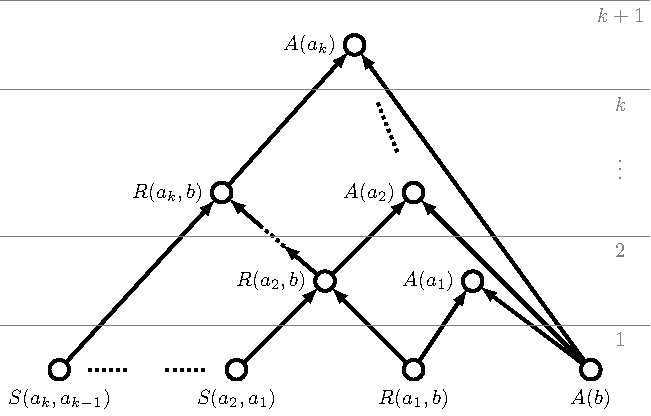
\includegraphics[width=0.7\textwidth]{fig-mg.eps}
\caption{An example of a materialization graph.}
\label{fig:mg}
\end{center}
\end{figure}

We say that a materialization graph $\mathcal{G}$ is a \emph{complete materialization graph}
when $\mathcal{G}$ contains all ground atoms in $T_R^{\omega}(\textbf{I})$.
The set of nodes in a complete materialization graph is actually the result
of materialization.
Thus, the procedure of materialization can be transformed into the construction of
a complete materialization graph.
In the remainder, we only consider complete materialization graphs and
do not distinguish the term from the
notion of `materialization graphs'.
It should also be noted that there may exist several materialization graphs for a datalog program.


\subsection{A Basic Parallel Algorithm}
\label{sec:alg-bsc}

In this part, we propose a parallel algorithm
(denoted by Algorithm~$\mathsf{A}_{bsc}$) that constructs a materialization graph for a given datalog program.
Our computational model is a PRAM (parallel, random-access machine) that is mostly used to analyze parallel
complexity. This model allows us to introduce \emph{the parallel assumption}:
for any datalog program $P=\langle R, \textbf{I}\rangle$,
any substitution of some atom and any rule instance in $P^*$ can be mapped to a unique memory
location; further, a one-to-one relation can be established between processors and rule instances.
Under this assumption, a processor can check the applicability of its corresponding
rule instance and access the state of an atom occurring in this rule instance in constant time.
Algorithm~$\mathsf{A}_{bsc}$ is then given as follows.\\


\noindent\texttt{Algorithm~$\mathsf{A}_{bsc}$}. Given a datalog program $P=\langle R, \textbf{I}\rangle$,
the algorithm returns a materialization graph $\mathcal{G}$ of $P$.
Suppose we have $|P^*|$ processors, and each rule instantiation in $P^*$ is
assigned to one processor.
Initially $\mathcal{G}$ is empty. The following three steps are then performed:
\begin{enumerate}[leftmargin=8ex,label=(\textit{Step \arabic*}),ref=Step~\arabic*]
\item Add all facts in $\textbf{I}$ to $\mathcal{G}$.\label{alg1:addFacts}
\item For each rule instantiation $B_1,...,B_n\rightarrow H$, if the body atoms are all
    in $\mathcal{G}$ while $H$ is not in $\mathcal{G}$,
    the corresponding processor adds $H$ to $\mathcal{G}$ and creates edges pointing
    from $B_1,...,B_n$ to $H$.\label{alg1:updateG}
\item If no processor can add more nodes and edges to $\mathcal{G}$,
  terminate, otherwise continue with \ref{alg1:updateG}.\label{alg1:halt}\hfill$\Box$
\end{enumerate}

\begin{example}
We consider the datalog program $P_{ex_1}$ in Example~\ref{exp:mg} again,
and perform Algorithm~$\mathsf{A}_{bsc}$ on it.
Initially, all the facts ($A(b),R(a_1,b),S(a_2,a_1),...,S(a_{k},a_{k-1})$) are added to the
result $\mathcal{G}_{ex_1}$ (\ref{alg1:addFacts}).
Then in different iterations of \ref{alg1:updateG}, the remaining nodes are added to
$\mathcal{G}_{ex_1}$ by different processors.
For example a processor $p$ is allocated a rule instantiation `$R(a_2,b),A(b)\rightarrow A(a_2)$'.
Then, processor $p$ adds $A(a_2)$ to $\mathcal{G}_{ex_1}$ after it checks that
$A(b)$ and $R(a_2,b)$ are in $\mathcal{G}_{ex_1}$.
Algorithm~$\mathsf{A}_{bsc}$ halts when $A(a_k)$ has been added to $\mathcal{G}_{ex_1}$ (\ref{alg1:halt}).
\end{example}

Lemma~\ref{lemma:a1} shows the correctness of Algorithm~$\mathsf{A}_{bsc}$ and that, for any datalog program $P$,
Algorithm~$\mathsf{A}_{bsc}$ always constructs a materialization graph with the minimum depth among all the
materialization graphs of $P$. The detailed proofs of Lemma~\ref{lemma:a1} and other lemmas and theorems can be found
in the appendix.

\begin{lemma}
\label{lemma:a1}
Given a datalog program $P=\langle R, \textbf{I}\rangle$, we have
\begin{enumerate}[leftmargin=4ex]
\item Algorithm~$\mathsf{A}_{bsc}$ halts and returns a materialization graph $\mathcal{G}$ of $P$;
\item $\mathcal{G}$ has the the minimum depth among all the materialization graphs of $P$.
\end{enumerate}
\end{lemma}

\begin{proof}[Proof sketch] This lemma can be proved by performing
an induction on $T_R^{\omega}(\textbf{I})$.
The stage (see the related contents in Section~\ref{sec:background}) of $P$
is the lower-bound of the depth of the materialization graphs. Based on the previous induction,
one can further check that, for the materialization graph $\mathcal{G}$ constructed by Algorithm~$\mathsf{A}_{bsc}$,
its depth equals the depth of the stage.
\end{proof}

We now discuss the parallel complexity of Algorithm~$\mathsf{A}_{bsc}$.
Given a class of datalog programs $\mathbb{P}$ where
a rule set is shared for each datalog program $P=\langle R, \textbf{I}\rangle$ in $\mathbb{P}$.
Let $e$, $v$ and $r$ represent the maximum arity of any EDB predicate, the maximum number of variables
in any datalog rule, and the number of datalog rules, respectively.
We then have that the number of
constants is at most $|\textbf{I}|e$, and the number of all possible rule instances in $P^*$
is at most $r(|\textbf{I}|e)^v$.
Note that $e, v$ and $r$ depend only on the rule set $R$ and not on the fact set $\textbf{I}$.
Thus, the memory space for storing the atoms and the rule instances is polynomial in the size of $\textbf{I}$.
This also means that the number of processors is polynomially bounded.
The computing time of \ref{alg1:addFacts} and \ref{alg1:halt} occupy constant time (denoted by $c_1$) because of parallelism.
Since Algorithm~$\mathsf{A}_{bsc}$ works under the parallel assumption, one iteration of
\ref{alg1:updateG} also costs constant time (denoted by $c_2$). Thus,
the whole computing time of Algorithm~$\mathsf{A}_{bsc}$ turns out to be $c_1+l\cdot c_2$
where $l$ denotes the number of iterations of \ref{alg1:updateG}.

An \texttt{NC} algorithm should meet two requirements: first,
it works on a polynomial number of processors; second, it halts in poly-logarithmic time.
As discussed above, Algorithm~$\mathsf{A}_{bsc}$ meets the first requirement.
If we want to restrict Algorithm~$\mathsf{A}_{bsc}$ to be an \texttt{NC} algorithm,
we can make the number of iterations of \ref{alg1:updateG} to be poly-logarithmically bounded.
We use the symbol $\psi$ to denote a poly-logarithmically bounded function.
For any datalog program, if we restrict the number of iterations of
\ref{alg1:updateG} to be bounded by $\psi(|\textbf{I}|)$,
the computing time of Algorithm~$\mathsf{A}_{bsc}$
is $c_1+\psi(|\textbf{I}|)\cdot c_2$. With this restriction, Algorithm~$\mathsf{A}_{bsc}$ is an \texttt{NC} algorithm denoted by
$\mathsf{A}_{bsc}^{\psi}$.

Based on $\mathsf{A}_{bsc}^{\psi}$, we can identify a class of datalog programs
$\mathcal{D}_{\mathsf{A}_{bsc}^{\psi}}$ such that all the datalog programs in it can be handled
by $\mathsf{A}_{bsc}^{\psi}$.
It is obvious that $\mathcal{D}_{\mathsf{A}_{bsc}^{\psi}}$ is a \texttt{PTD} class.
We use the following theorem to further show that this class can be captured based on
the materialization graphs of the datalog programs in $\mathcal{D}_{\mathsf{A}_{bsc}^{\psi}}$.

\begin{theorem}\label{theorem:a1}
For any datalog program $P$, $P\in\mathcal{D}_{\mathsf{A}_{bsc}^{\psi}}$ iff $P$ has a
materialization graph whose depth is upper-bounded by $\psi(|P|)$.
\end{theorem}

\begin{proof}[Proof sketch]
We can first prove that the number of iterations
of \ref{alg1:updateG} is actually the depth of the constructed materialization
graph. This theorem then follows by considering
Lemma~\ref{lemma:a1}.
\end{proof}

Consider Example~\ref{exp:mg} again. Let the integer $k$ be a variable. We can
get a class of datalog programs, denoted by $\mathbb{P}_{ex_1}$, where the rule set
is $\{R(x,y),A(y)\rightarrow A(x), S(x,y),R(y,z)\rightarrow R(x,z)\}$ and the fact
set varies according to $k$. The algorithm $\mathsf{A}_{bsc}^{\psi}$ is restricted in the sense that it cannot even work on the rather simple datalog program class $\mathbb{P}_{ex_1}$.
Let $\mathcal{G}_{ex_1}$ be some materialization graph corresponding
to some datalog program in $\mathbb{P}_{ex_1}$. It can be checked that
\texttt{depth}($\mathcal{G}_{ex_1}$)$=k$ for some $k$.
This means that the depths of the materialization graphs are linearly bounded by $k$.
On the other hand, the sizes of the datalog programs in $\mathbb{P}_{ex_1}$ are polynomial in $k$.
Thus, for any $\psi$ that is poly-logarithmically bounded, we can always find a $k$ large
enough such that $\mathsf{A}_{bsc}^{\psi}$ terminates without constructing a materialization
graph for each datalog program in $\mathbb{P}_{ex_1}$.
However, there indeed exists an \texttt{NC} algorithm that can handle $\mathbb{P}_{ex_1}$.
We discuss this in the next part.


\subsection{Optimizing Algorithm~$\mathsf{A}_{bsc}$ via Single-Way Derivability}

In this part, we optimize Algorithm~$\mathsf{A}_{bsc}$ such that $P_{ex_1}$
can be handled. Based on the optimized variant of Algorithm~$\mathsf{A}_{bsc}$,
we can identify another \texttt{PTD} class.

We discuss our optimization based on a specific case in Example~\ref{exp:general}.
We find that, in this kind of case, the construction of a materialization graph can be accelerated.

\begin{figure}[htbp]
\begin{center}
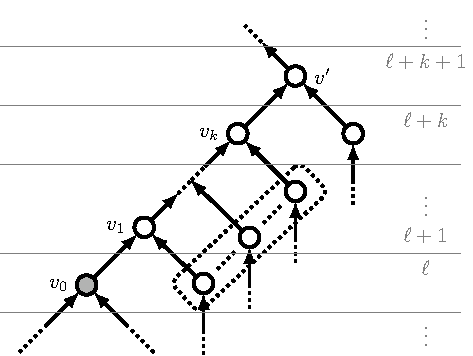
\includegraphics[width=0.7\textwidth]{fig-general.eps}
\caption{A partial materialization graph}
\label{fig:general}
\end{center}
\end{figure}

\begin{example}\label{exp:general}
Consider the  snapshot of Algorithm~$\mathsf{A}_{bsc}$ in
Figure~\ref{fig:general}. A materialization graph $\mathcal{G}$
is being constructed for some datalog program $\langle R, \textbf{I}\rangle$.
The nodes in the dashed box denote the ones that have been added to $\mathcal{G}$.
In this snapshot, $v_0$ has been newly added
to $\mathcal{G}$ in the $\ell^{th}$ ($\ell\geq 1$) iteration.
Each of the nodes $v_i$ ($1\leq i\leq k$) has at most one parent node not in $\mathcal{G}$,
while $v'$ has two parent nodes not in $\mathcal{G}$.
All of the nodes $v_i$ ($1\leq i\leq k$) and $v'$ would be added to $\mathcal{G}$
afterwards.
\end{example}


In Example~\ref{exp:general}, $v_k$ would be added to $\mathcal{G}$ after \emph{at least} $k$
iterations by performing Algorithm~$\mathsf{A}_{bsc}$.
We can check that each edge $(v_{i-1},v_i)$ ($1\leq i\leq k$) in this
stage adheres to the condition:
\emph{if the parent node $v_{i-1}$ is derivable, the child node $v_i$ is derivable} (this
is because for a node $v_i$, the node $v_{i-1}$ is the only parent node that has not been added to $\mathcal{G}$).
We call this condition the \emph{single-way derivability condition}, which intuitively says that the derivability of a
node only depends on one of its parent nodes.
Observe that node $v_k$ is reachable from node $v_0$ through the path $\tau=(v_0,v_1,\ldots,v_k)$ where
each edge $(v_{i-1},v_i)$ ($1\leq i\leq k$) satisfies the single-way derivability condition.
We call such a path a \emph{single-way derivable} (SWD) path.
Further, the starting node $v_0$ in $\tau$ has been added to $\mathcal{G}$; in other words,
$v_0$ is derivable. Thus, all of the nodes $v_i$ ($1\leq i\leq k$) can be added to
$\mathcal{G}$ immediately.
Based on the above idea, we optimize Algorithm~$\mathsf{A}_{bsc}$ by checking whether such an SWD path
exits for some node $v$. If there is an SWD path for node $v$, this node can be added to $\mathcal{G}$
due to the single-way derivability condition.

For Example~\ref{exp:general},
there exists an SWD path $(v_0,\ldots,v_i)$ for each node $v_i$
($1\leq i\leq k$), hence, all of these nodes
can be added to $\mathcal{G}$ right after $v_0$. On the other hand,
node $v'$ has no SWD path since it has two parent nodes not in $\mathcal{G}$.

We next discuss how to determine the existence of SWD paths. Note that, SWD paths require us to
describe the reachability between two nodes. To this extent, we use a
binary transitive relation $\texttt{rch} \subseteq T_R^{\omega}(\textbf{I})\times T_R^{\omega}(\textbf{I})$,
e.g., \texttt{rch}$(v_1,v_2)$ means that $v_2$ is reachable from $v_1$.
In each iteration of \ref{alg1:updateG} in Algorithm~$\mathsf{A}_{bsc}$, we further compute a \texttt{rch}
relation (denoted by $S_{\textit{\tiny rch}}$) by performing the following process:

\begin{description}[leftmargin=4ex]
\item[(\textbf{\dag})] \emph{For each rule instantiation of the form $B_1,..,B_i,..,B_n\rightarrow H$
such that $H$ has not been added to $\mathcal{G}$}:
\begin{enumerate}[leftmargin=0ex]
\item \emph{if the all body atoms $B_1,...,B_n$ have been added to $\mathcal{G}$, put \texttt{rch}$(B_1,H),...,$ \texttt{rch}$(B_n,H)$ in $S_{\textit{\tiny rch}}$};
\item \emph{if $B_i$ is the only node in the body that has not been added to $\mathcal{G}$,
    put \texttt{rch}$(B_i,H)$ in $S_{\textit{\tiny rch}}$}.\hfill$\Box$
\end{enumerate}
\end{description}

We then compute the transitive closure (denoted by $S^*_{\!\textit{\tiny rch}}$) with respect to
$S_{\!\textit{\tiny rch}}$. Based on the transitive closure, we can
perform the following optimization: 
for a node $v$, if there is a relation $\texttt{rch}(v',v)\in S^*_{\!\textit{\tiny rch}}$
such that $v'$ has been added to $\mathcal{G}$ and $v$ has an SWD
path, then $v$ can be added to $\mathcal{G}$.
The following algorithm applies this optimization strategy.\\

\noindent\texttt{Algorithm~$\mathsf{OPT}$}. The algorithm requires two inputs:
a datalog program $P=\langle R, \textbf{I}\rangle$ and a (partial) materialization graph $\mathcal{G}$ that is
being constructed from $P$. The following steps are performed:
\begin{enumerate}[leftmargin=6ex,label=(\textbf{\roman*})]
\item Compute a \texttt{rch} relation $S_{\!\textit{\tiny rch}}$ by following the above process (see $(\textbf{\dag})$).\label{rch}
\item Compute the transitive closure $S^*_{\!\textit{\tiny rch}}$ of $S_{\!\textit{\tiny rch}}$.\label{transClos}
\item Update $\mathcal{G}$ as follows: for any \texttt{rch}$(B_i,H)\in S_{\!\textit{\tiny rch}}$
that corresponds to `$B_1,..,B_i,..$ $,B_n\rightarrow H$'
    and there exists a node $B'$ such that \texttt{rch}$(B',B_i)\in S^*_{\!\textit{\tiny rch}}$ and $B'$ is
    in $\mathcal{G}$; if $H$ is not in $\mathcal{G}$ or $H$ is in $\mathcal{G}$ but has no parent pointing
    to it, add $H$ and $B_i$ (if $B_i$ is not in $\mathcal{G}$) to $\mathcal{G}$, and create the edges
    $e(B_1, H),...,e(B_n, H)$ in $\mathcal{G}$. Do nothing for other statements
    \texttt{rch}$(B_j,H)\in S_{\!\textit{\tiny rch}}$.\label{updateG}\hfill$\Box$
\end{enumerate}

It is well known that there is an \texttt{NC} algorithm for computing the
transitive closure \cite{Allender07}.
Based on this result and Algorithm~$\mathsf{OPT}$, we propose an optimized variant of Algorithm~$\mathsf{A}_{bsc}$:\\

\noindent\texttt{Algorithm~$\mathsf{A}_{opt}$}. Given a datalog program $P=\langle R, \textbf{I}\rangle$, the algorithm
returns a materialization graph $\mathcal{G}$ of $P$.
Suppose we have $|P^*|$ processors, and each rule instantiation in $P^*$ is
assigned to one processor.
Initially $\mathcal{G}$ is empty. The following steps are then performed:
\begin{enumerate}[leftmargin=8ex,label=(\textit{Step \arabic*}),ref=Step~\arabic*]
\item Add all facts in $\textbf{I}$ to $\mathcal{G}$.\label{alg3:addFacts}
\item Compute $S_{\!\textit{\tiny rch}}$ by performing \ref{rch} in Algorithm~$\mathsf{OPT}$; use an \texttt{NC}
    algorithm to compute the transitive closure $S^*_{\!\textit{\tiny rch}}$ (see \ref{transClos} in Algorithm~$\mathsf{OPT}$);
    update $\mathcal{G}$ by performing \ref{updateG}  in Algorithm~$\mathsf{OPT}$.\label{alg3:updateG}
\item If no node has been added to $\mathcal{G}$ (in \ref{alg3:updateG}), terminate,
    otherwise iterate \ref{alg3:updateG}. \label{alg3:halt}\hfill$\Box$
\end{enumerate}

It should be noted that there has to be an SWD path for any derivable node in some iteration when performing
Algorithm~$\mathsf{A}_{opt}$.
The following lemma shows the correctness of Algorithm~$\mathsf{A}_{opt}$.

\begin{lemma}\label{lemma:a3}
Given a datalog program $P=\langle R, \textbf{I}\rangle$,
$\mathsf{A}_{opt}$ halts and outputs a materialization graph $\mathcal{G}$ of $P$.
\end{lemma}

\begin{example}\label{exp:opt}
We perform Algorithm~$\mathsf{A}_{opt}$ on the datalog program $P_{ex_1}$ in Example~\ref{exp:mg}.
Initially, $R(a_1,b)$ is in the materialization graph $\mathcal{G}_{ex_1}$.
In the first iteration of \ref{alg3:updateG}, all the rule instantiations are in two kinds of forms:
`$R(a_i,b),A(b)\rightarrow A(a_i)$' and `$S(a_i,a_{i-1}),$ $R(a_{i-1},b)\rightarrow R(a_i,b)$' $(2\leq i\leq k)$,
$S_{\!\textit{\tiny rch}}$ is the set $\{$\texttt{rch}$(R(a_{i-1},b), R(a_i,b))|2\leq i\leq k\}
\cup\{$\texttt{rch}$(R(a_i,b), A(a_i))|1\leq i\leq k\}$.
In the transitive closure of $S_{\!\textit{\tiny rch}}$,
one can check that \texttt{rch}$(R(a_1,b), R(a_i,b)),$
\texttt{rch}$(R(a_1,b), A(a_i))\in S^*_{\!\textit{\tiny rch}}(2\leq i\leq k)$.
Thus, $R(a_i,b)$ and $A(a_i)$ ($2\leq i\leq k$) can all be added to $\mathcal{G}_{ex_1}$
in the first iteration of \ref{alg3:updateG}.
\end{example}

The analysis of the parallel complexity of Algorithm~$\mathsf{A}_{opt}$ is given as follows.
We use the same symbols $e$, $v$ and $r$ that are used for analyzing the complexity of Algorithm~$\mathsf{A}_{bsc}$
(see Section~\ref{sec:alg-bsc}). Similarly to the analysis for Algorithm~$\mathsf{A}_{bsc}$, it can be checked that
the number of processors is polynomial of $|\textbf{I}|$, i.e., $r(|\textbf{I}|e)^v$.
We now consider the computing time of Algorithm~$\mathsf{A}_{opt}$. It is obvious that \ref{alg3:addFacts}
\ref{alg3:halt} occupy constant time (denoted by $c_1$). In \ref{alg3:updateG}, the phases of
computing $S_{\!\textit{\tiny rch}}$ and updating $\mathcal{G}$ also take constant time (denoted by $c_2$)
under the parallel assumption. Recall that the number of constants is at most $|\textbf{I}|e$ (see Section~\ref{sec:alg-bsc}).
Let $w$ and $p$ represent the maximum arity of any predicate and the number of predicates respectively.
We have that the number of all possible substitutions of atoms is at most $p(|\textbf{I}|e)^w$.
The relation $S_{\!\textit{\tiny rch}}$ consists of pairs of the atoms. Thus, the size of $S_{\!\textit{\tiny rch}}$
is bounded by $p^2(|\textbf{I}|e)^{2w}$. It can be checked that the computing time of the \texttt{NC} algorithm for computing the transitive
closure of $S_{\!\textit{\tiny rch}}$ is poly-logarithmical in the size of $\textbf{I}$, more precisely,
it is upper bounded to $\log^2(p^2(|\textbf{I}|e)^{2w})$ ($=4\log^2(p)+4w^2\log^2(|\textbf{I}|e)+8w\log(p)\log(|\textbf{I}|e)$).
We now have that the total computing time of Algorithm~$\mathsf{A}_{opt}$ is $c_1+lc_3 + lc_4\log(|\textbf{I}|e) +lc_5\log^2(|\textbf{I}|e)$
where $c_3=c_2+4\log^2(p)$, $c_4=8w\log(p)$, $c_5=4w^2$ and $l$ denotes the number of iterations of \ref{alg3:updateG}.

Algorithm~$\mathsf{A}_{opt}$ can be restricted to an \texttt{NC} algorithm analogously to the process
for Algorithm~$\mathsf{A}_{bsc}$. That is the number of iterations of \ref{alg3:updateG}
is poly-logarithmically bounded, i.e., it is bounded by $\psi(|\textbf{I}|)$
where $\psi$ is a poly-logarithmical function. In this way, the computing time of
Algorithm~$\mathsf{A}_{bsc}$ turns out to be $c_1+c_3\psi(|\textbf{I}|)+c_4\psi(|\textbf{I}|)\log(|\textbf{I}|e)+
c_5\psi(|\textbf{I}|)\log^2(|\textbf{I}|e)$,
which is still poly-logarithmical in the size of $\textbf{I}$. We denote the
\texttt{NC} variant of Algorithm~$\mathsf{A}_{opt}$ by $\mathsf{A}_{opt}^{\psi}$.

Based on $\mathsf{A}_{opt}^{\psi}$, we can identify a \texttt{PTD} class $\mathcal{D}_{\mathsf{A}_{opt}^{\psi}}$.
Further, we have the following corollary which implies that $\mathsf{A}_{opt}^{\psi}$ performs better
than $\mathsf{A}_{bsc}^{\psi}$ in terms of computing time.

\begin{corollary}
For any poly-logarithmically bounded function $\psi$,
we have that $\mathcal{D}_{\mathsf{A}_{bsc}^{\psi}}\subseteq\mathcal{D}_{\mathsf{A}_{opt}^{\psi}}$.
\end{corollary}

\begin{proof}[Proof sketch]
Suppose $P\in\mathcal{D}_{\mathsf{A}_{bsc}^{\psi}}$. According to Theorem~\ref{theorem:a1},
the depth of the materialization graph $\mathcal{G}$ constructed by $\mathsf{A}_{bsc}^{\psi}$ is upper-bounded by $\psi(|P|)$.
It is obvious that the number of nodes in each path of $\mathcal{G}$ is also upper-bounded by $\psi(|P|)$.
According to the optimization strategy applied in $\mathsf{A}_{opt}$, if $\mathcal{G}$ can be constructed
by $\mathsf{A}_{opt}$, the number of iterations of $\mathsf{A}_{opt}$ has to be upper-bounded by $\psi(|P|)$;
if $\mathcal{G}$ is not the materialization graph constructed
by $\mathsf{A}_{opt}$, then there has to exist another materialization graph $\mathcal{G}'$ constructed by $\mathsf{A}_{opt}$
and $\mathcal{G}'$ has a smaller depth compared with $\mathcal{G}$.
\end{proof}



%%% Local Variables:
%%% mode: latex
%%% TeX-master: "parallel-tractability-J"
%%% End:


\section{Parallel Tractability of Ontology Materialization in OWL}
\label{sec:ptonto}

In this section, we study the issue of parallel tractability
for materialization of DL-Lite and DHL (DHL($\circ$)) ontologies
based on Algorithm~$\mathsf{A}_{\text{opt}}$. We show that, for any class $\mathbb{O}$ of
DL-Lite$_{\text{core}}$ or DL-Lite$_\mathcal{R}$ ontologies,
there exists a poly-logarithmically bounded function $\psi$
such that Algorithm~$\mathsf{A}_{\text{opt}}^{\psi}$ can handle materialization of the ontologies in $\mathbb{O}$.
However, for DHL and DHL($\circ$), there exist ontology classes such that Algorithm~$\mathsf{A}_{\text{opt}}^\psi$
does not work. We illustrate the reason why Algorithm~$\mathsf{A}_{\text{opt}}^\psi$ cannot always
work by studying specific cases.
Further, we propose to restrict the usage of DHL and DHL($\circ$) in order to achieve parallel tractability
of materialization.

\subsection{Materialization of DL-Lite Ontologies via Algorithm~$\mathsf{A}_{\text{opt}}$}

In this part, we show how to use Algorithm~$\mathsf{A}_{\text{opt}}$ to handle
DL-Lite materialization and analyze its parallel tractability.
Based on the analysis, we have that, for any DL-Lite$_{\text{core}}$ or DL-Lite$_\mathcal{R}$ ontology
there always exists an SWD path for each atom of the form $A(a)$ or $R(a,b)$.
In other words, all atoms of the forms $A(a)$ and $R(a,b)$ can be added to
the constructed materialization graph in the first iteration of \ref{alg3:updateG}
by performing Algorithm~$\mathsf{A}_{\text{opt}}$.

In order to show how Algorithm~$\mathsf{A}_{\text{opt}}$ handles DL-Lite materialization,
we use the following example.

\begin{example}\label{exp:dllite}
Given a DL-Lite ontology $\mathcal{O}_{\text{ex}_5}$
where the TBox and RBox contain the following axioms:
$A\sqsubseteq B_1$, $A\sqsubseteq B_2$, $B_1\sqcap B_2\sqsubseteq\bot$,
$\exists R.B_2\sqsubseteq\bot$, $Q\sqsubseteq S^-$, $\exists Q.\top\sqsubseteq A$ and $S\sqsubseteq R$;
its ABox contains an assertion $Q(a,b)$.
We denote the corresponding datalog program of $\mathcal{O}_{\text{ex}_5}$ by $P_{\text{ex}_5}=\langle R, \textbf{I}\rangle$,
where $R$ contains the rules that are transformed from the above axioms; $\textbf{I}$ contains $Q(a,b)$
as the only fact.
The unique materialization graph of $P_{\text{ex}_5}$ is denoted by
$\mathcal{G}_{\text{ex}_5}$ (see
Figure~\ref{fig:ex2}).
\end{example}

\begin{figure}[htbp]
\begin{center}
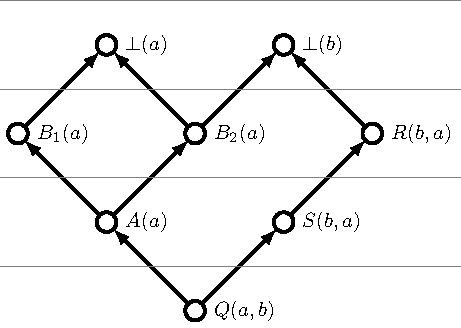
\includegraphics[width=0.5\textwidth]{fig-dllite.pdf}
\caption{The materialization graph of $\mathcal{O}_{\text{ex}_5}$}
\label{fig:ex2}
\end{center}
\end{figure}

Consider performing Algorithm~$\mathsf{A}_{\text{opt}}$ on the ontology $\mathcal{O}_{\text{ex}_5}$ in Example~\ref{exp:dllite}.
(\uppercase\expandafter{\romannumeral1}) First, Algorithm~$\mathsf{A}_{\text{opt}}$ adds all ABox assertions (only $Q(a,b)$ here)
to the initially empty graph $\mathcal{G}_{\text{ex}_5}$ (\ref{alg3:addFacts} of Algorithm~$\mathsf{A}_{\text{opt}}$).
(\uppercase\expandafter{\romannumeral2}) In the first iteration of
\ref{alg3:updateG}, Algorithm~$\mathsf{A}_{\text{opt}}$ checks that all of the nodes
$A(a)$, $S(b,a)$, $B_1(a)$, $B_2(a)$ and $R(b,a)$ have corresponding SWD paths
starting from $Q(a,b)$. Thus, Algorithm~$\mathsf{A}_{\text{opt}}$
adds these nodes to $\mathcal{G}_{\text{ex}_5}$ immediately. We take an example of node $B_1(a)$,
for which an SWD path $(Q(a,b),A(a),B_1(a))$ exists.
When updating $\mathcal{G}_{\text{ex}_5}$ by adding $B_1(a)$ to it,
Algorithm~$\mathsf{A}_{\text{opt}}$ first checks whether the parent node $A(a)$ of $B_1(a)$
has been in $\mathcal{G}_{\text{ex}_5}$; if $A(a)$ is already in $\mathcal{G}_{\text{ex}_5}$, $B_1(a)$
is added to $\mathcal{G}_{\text{ex}_5}$ by creating an edge pointing from $A(a)$ to $B_1(a)$;
if $A(a)$ has not been added to $\mathcal{G}_{\text{ex}_5}$,
Algorithm~$\mathsf{A}_{\text{opt}}$ adds $A(a)$ ($B_1(a)$, respectively)
to $\mathcal{G}_{\text{ex}_5}$ and creates an edge pointing from
$Q(a,b)$ to $A(a)$ (an edge pointing from $A(a)$ to $B_1(a)$, respectively).\footnote{These two cases may happen simultaneously,
since node $A(a)$ and node $B_1(a)$ are being processed in parallel.} The other nodes
$A(a)$, $S(b,a)$, $B_2(a)$ and $R(b,a)$ are processed similarly.
(\uppercase\expandafter{\romannumeral3})
The two nodes $\bot(a)$ and $\bot(b)$
have no SWD path in the first iteration of \ref{alg3:updateG}.
They are left to be processed in the second iteration.
(\uppercase\expandafter{\romannumeral4})
Finally, Algorithm~$\mathsf{A}_{\text{opt}}$ finishes constructing $\mathcal{G}_{\text{ex}_5}$
after two iterations (\ref{alg3:halt}).

From the above example, we can observe that SWD paths exist
for all nodes except $\bot(a)$ and $\bot(b)$ in the first iteration of Algorithm~$\mathsf{A}_{\text{opt}}$.
Further, we give the following lemma that holds for any DL-Lite$_{\text{core}}$ or DL-Lite$_\mathcal{R}$ ontology.

\begin{lemma}\label{lemma:dllite}
For any DL-Lite$_{\text{core}}$ or DL-Lite$_\mathcal{R}$ ontology $\mathcal{O}$, there exists a materialization graph $\mathcal{G}$ such that
each atom of the form $A(x)$ ($A\neq\bot$) or $R(x,y)$ in $\mathcal{G}$ has an SWD path.
\end{lemma}

The above lemma guarantees that all atoms of the form $A(x)$ ($A\neq\bot$) or $R(x,y)$
have to be added to the constructed materialization graph in the first iteration of
\ref{alg3:updateG} by applying Algorithm~$\mathsf{A}_{\text{opt}}$.
For each atom of the form $\bot(x)$, there may not exist an SWD path in the first iteration
of \ref{alg3:updateG}, since its derivability depends on its two parent nodes
(see nodes $\bot(a)$ and $\bot(b)$ in $\mathcal{G}_{\text{ex}_5}$ of
Example~\ref{exp:dllite}). On the other hand, according to the syntax of DL-Lite,
$\bot$ does not occur on the left-hand side of any axiom. In other words,
an atom of the form $\bot(x)$ cannot be the parent of any other node.
This allows for adding all atoms of the form $\bot(x)$ to the constructed materialization graph in at most two iterations of
\ref{alg3:updateG} by applying Algorithm~$\mathsf{A}_{\text{opt}}$.
Based on the above discussion, for any DL-Lite ontology $\mathcal{O}$,
there always exists a poly-logarithmically bounded function $\psi$ such that
Algorithm~$\mathsf{A}_{\text{opt}}^{\psi}$ can handle the materialization of $\mathcal{O}$;
more precisely, we can set that $\psi=2$. This result is consistent with
that by \citet{CalvaneseGLLR07}.
Formally, we use $\mathcal{D}_{\textit{dl\_lite}}$
to denote the set of all DL-Lite$_{\text{core}}$ and DL-Lite$_\mathcal{R}$ ontologies and give the following theorem.

\begin{theorem}\label{theorem:dl-lite}
There exists a poly-logarithmically bounded function $\psi$ such that
$\mathcal{D}_{\textit{dl\_lite}}\subseteq\mathcal{D}_{\mathsf{A}_{\text{opt}}^{\psi}}$.
\end{theorem}


\subsection{Parallel Tractability of  DHL Materialization}
\label{sec:DHL}

In this part, we study whether Algorithm~$\mathsf{A}_{\text{opt}}^\psi$ can handle DHL ontologies.
Unfortunately there exist DHL ontology classes such that Algorithm~$\mathsf{A}_{\text{opt}}^\psi$
does not work for any poly-lo\-ga\-rith\-mi\-cal\-ly bounded function $\psi$.
In the following, we first give such a case
to illustrate the reason why Algorithm~$\mathsf{A}_{\text{opt}}^\psi$ cannot work.
Based on the analysis of this case, we propose to restrict
the usage of DHL in order to achieve parallel tractability
of materialization.

We find that, an unlimited usage of axioms of the
form $B_1\sqcap B_2\sqsubseteq A$
makes it impossible for Algorithm~$\mathsf{A}_{\text{opt}}$ to construct a materialization graph
in a poly-logarithmic number of iterations of \ref{alg3:updateG}.
We use the following example to illustrate this.

\begin{figure}[htbp]
\begin{center}
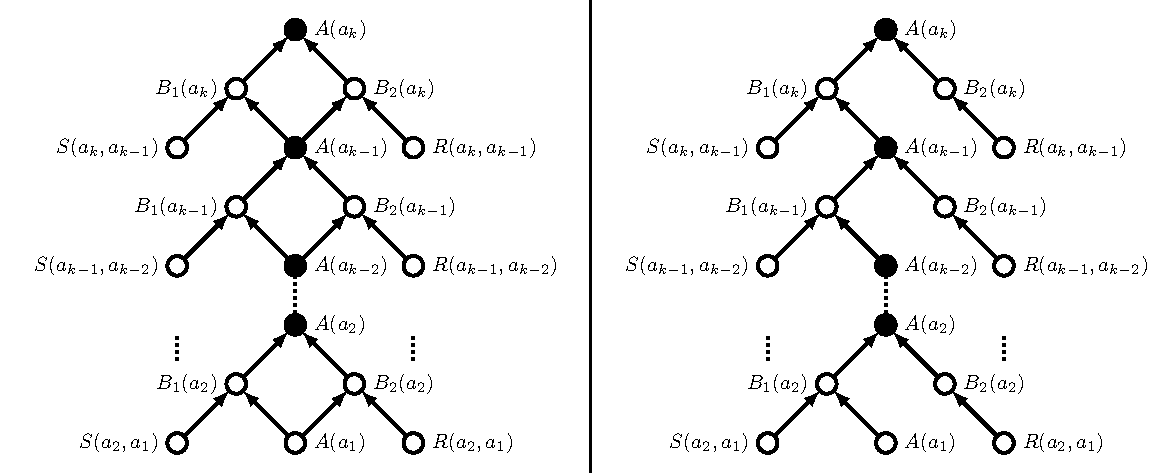
\includegraphics[width=\textwidth]{fig-pathtwist.pdf}
\caption{The materialization graph of $\mathcal{O}_{\text{ex}_6}$
  (left) and of $\mathcal{O}_{\text{ex}_7}$ (right)}
\label{fig:ex3_4}
\end{center}
\end{figure}

\begin{example}\label{exp:dhl}
Given a DHL ontology $\mathcal{O}_{\text{ex}_6}$ where the TBox contains three axioms:
$B_1\sqcap B_2\sqsubseteq A$, $\exists S.A\sqsubseteq B_1$ and $\exists R.A\sqsubseteq B_2$;
the ABox is $\{S(a_i,a_{i-1}), R(a_i,a_{i-1}), A(a_1)\}$
for $2\leq i\leq k$ and $k$ an integer greater than $2$.
We denote the corresponding datalog program of $\mathcal{O}_{\text{ex}_6}$ by $P_{\text{ex}_6}=\langle R, \textbf{I}\rangle$,
where $R$ contains three rules: `$B_1(x),B_2(x)\rightarrow A(x)$',`$S(x,y),A(y)\rightarrow B_1(x)$' and `$R(x,y),A(y)\rightarrow B_2(x)$'.
The materialization graph of $P_{\text{ex}_6}$ constructed by
$\mathsf{A}_{\text{opt}}$ is denoted by $\mathcal{G}_{\text{ex}_6}$
(see Figure~\ref{fig:ex3_4}~(left)).
\end{example}

One can check that $\mathcal{G}_{\text{ex}_6}$ is the unique materialization graph of $P_{\text{ex}_6}$.
Observe that there exists a path (e.g., $A(a_1),B_1(a_2),A(a_2),\ldots,A(a_k)$) between $A(a_1)$ and $A(a_k)$.
When performing Algorithm~$\mathsf{A}_{\text{opt}}$ on $P_{\text{ex}_6}$, it can be checked that
each node of the form $A(a_i)$ (filled with black color,
and $2\leq i\leq k$) has no SWD path until the $i^{th}$ iteration;
in the $i^{th}$ iteration, the parent nodes of $A(a_i)$ have been added to $\mathcal{G}_{\text{ex}_6}$,
and, $A(a_i)$ can also be added to $\mathcal{G}_{\text{ex}_6}$.
Similar to the datalog program class $\mathbb{P}_{\text{ex}_1}$, we can also get a
datalog program class $\mathbb{P}_{\text{ex}_6}$ for the ontology $\mathcal{O}_{\text{ex}_6}$
when $k$ is a variable. Based on the above analysis, Algorithm~$\mathsf{A}_{\text{opt}}$ cannot complete the materialization
for the datalog programs of $\mathbb{P}_{\text{ex}_6}$ in a poly-logarithmic
number of iterations.
The intuitive reason is that at least two paths exist
from $A(a_1)$ to $A(a_k)$. These paths \emph{twist} mutually and share the same joint nodes (see the black nodes).
This invalidates the optimization used in Algorithm~$\mathsf{A}_{\text{opt}}$.
That is, for each node $A(a_i)$, $2\leq i\leq k$, until its parents ($B_1(a_i)$ and $B_2(a_i)$) are added
to $\mathcal{G}_{\text{ex}_6}$, there would not exist an available SWD path for $A(a_i)$.
We use the term `\emph{path twisting}' to refer to such cases.

In order to make Algorithm~$\mathsf{A}_{\text{opt}}$ terminate in a poly-logarithmic number of iterations,
we consider restricting the usage of axioms of the form $B_1\sqcap B_2\sqsubseteq A$
to avoid `path twisting'. An intuitive idea is to
ensure that \emph{there is only one path between each two atoms of the form $A(x)$
generated from the rules corresponding to (T1)}.
We explain it by using the following example where the ontology is modified from
that in Example~\ref{exp:dhl}.

\begin{example}\label{exp:simpleC}
Consider an ontology $\mathcal{O}_{\text{ex}_7}$ where the TBox contains three axioms:
$B_1\sqcap B_2\sqsubseteq A$, $\exists S.A\sqsubseteq B_1$ and $B_3\sqsubseteq B_2$;
the ABox is $\{S(a_i,a_{i-1}), B_3(a_i), A(a_1)\}$
for $2\leq i\leq k$ and $k$ an integer greater than $2$.
We denote the corresponding datalog program by $P_{\text{ex}_7}$ where the rule set contains:
`$B_1(x),B_2(x)\rightarrow A(x)$',`$S(x,y),A(y)\rightarrow B_1(x)$' and `$B_3(x)\rightarrow B_2(x)$'.
$P_{\text{ex}_7}$ has a unique materialization graph denoted by $\mathcal{G}_{\text{ex}_7}$ (see Figure~\ref{fig:ex3_4}~(right)).
\end{example}

In the above example, for the axiom $B_1\sqcap B_2\sqsubseteq A$, all derived atoms
of the form $B_2(x)$ must not be child nodes of an atom $A(y)$ for some $y$.
This ensures that only one path exists between each two nodes among $A(a_2),\ldots,A(a_k)$.
Further, when constructing $\mathcal{G}_{\text{ex}_7}$, Algorithm~$\mathsf{A}_{\text{opt}}$ can terminate after
two iterations of \ref{alg3:updateG}. Specifically, in the first iteration, Algorithm~$\mathsf{A}_{\text{opt}}$
adds all of the nodes $B_3(a_i)$ and $B_2(a_i)$, $2\leq i\leq k$, to $\mathcal{G}_{\text{ex}_7}$
since they have corresponding SWD paths;
after that, all other nodes
can be added to $\mathcal{G}_{\text{ex}_7}$ in the second iteration (because each
node has an SWD path).
Motivated by this example, we consider restricting the usage of
the axioms $B_1\sqcap B_2\sqsubseteq A$
such that all atoms of the form $B_1(x)$ or $B_2(x)$ cannot be generated by an atom $A(y)$
for some $y$.
To this end, we first define \emph{simple concepts} as follows:

\begin{definition}
Given an ontology $\mathcal{O}=\langle\mathcal{T},\mathcal{R},\mathcal{A}\rangle$,
a concept $A\in\textbf{CN}$ is simple, if (1) $A$ does not occur on the right-hand side
of some axiom; or (2) $A$ satisfies the following conditions:
\begin{enumerate}[leftmargin=4ex,label=\arabic*.]
\item for each $B\sqsubseteq A\in\mathcal{T}$, $B$ is simple;
\item for each $\exists R.B\sqsubseteq A\in\mathcal{T}$, $B$ is simple;
\item there is no axiom of the form $B_1\sqcap B_2\sqsubseteq A$ in $\mathcal{T}$.
\end{enumerate}
\end{definition}

Based on simple concepts, we restrict DHL ontologies such that, in all axioms of the
form $B_1\sqcap B_2\sqsubseteq A$, at least one concept of $B_1$ and $B_2$ should be a simple concept
(we call this the \emph{simple-concept restriction}).
Intuitively, for such restricted DHL ontologies, the situation of `path twisting' does not happen.
This is because, for each axiom of the form $B_1\sqcap B_2\sqsubseteq
A$ such that, w.l.o.g., $B_1$
is a simple concept, none of the ancestors of $B_1(x)$ for some $x$
is generated from the rules corresponding to (T1).

\begin{example}
In the ontology of Example~\ref{exp:dhl}, all of $A$, $B_1$ and $B_2$ are
non-simple concepts.
In the ontology of Example~\ref{exp:simpleC}, $A$ and $B_1$ are non-simple concepts,
while $B_3$ and $B_2$ are simple concepts. Further, it can be checked that
the ontology  of Example~\ref{exp:simpleC} follows the simple-concept restriction
and can be handled by Algorithm~$\mathsf{A}_{\text{opt}}^\psi$ for some poly-logarithmic function $\psi$.
\end{example}

We define the following class of DHL ontologies based on the above restriction and
give Theorem \ref{theorem:dhl} to show that any DHL ontology that satisfies the
simple-concept restriction can be handled by Algorithm~$\mathsf{A}^\psi_{\text{opt}}$
for some poly-logarithmic function $\psi$.

\begin{definition} Let $\mathcal{D}_{\textit{\text{dhl}}}$ be a class of datalog programs where
each program is rewritten from a DHL ontology that follows the condition that, for all axioms of the form
$A_1\sqcap A_2\sqsubseteq B$, at least one concept of $A_1$ and $A_2$ should be a \emph{simple concept}.
\end{definition}

\begin{theorem}\label{theorem:dhl}
There exists a poly-logarithmically bounded function $\psi$ s.t.
$\mathcal{D}_{\textit{\text{dhl}}}\subseteq\mathcal{D}_{\mathsf{A}_{\text{opt}}^{\psi}}$.
\end{theorem}


\subsection{Parallel Tractability of DHL($\circ$) Materialization}
\label{sec:DHLo}

In this part, we study materialization tractable in parallel for DHL($\circ$) ontologies.
In addition to the rules in DHL, we also have to consider complex RIAs (R4).
We next show that complex RIAs may also cause the situation of `path twisting'.
Consider the following example:
%
\begin{example}\label{exp:complexRIA}
Given a DHL$(\circ)$ ontology $\mathcal{O}_{\text{ex}_9}$ where the TBox is empty;
the RBox $\mathcal{R}$ contains three axioms:
$R_1\circ R_2\sqsubseteq R$, $R_3\circ R\sqsubseteq R_1$ and $R\circ R_4\sqsubseteq R_2$;
the ABox $\mathcal{A}$ is $\{R(a_1,a_1), R_3(a_i,a_{i-1}), R_4(a_{i-1},a_i)\}$
for $2\leq i\leq k$ and $k$ an integer greater than $2$.
The corresponding datalog program $P_{\text{ex}_9}$
contains three rules: `$R_1(x,y),R_2(y,z)\rightarrow R(x,z)$',
`$R_3(x,y),R(y,z)\rightarrow R_1(x,z)$' and `$R(x,y),R_4(y,z)\rightarrow R_2(x,z)$'.
The materialization graph of $P_{\text{ex}_9}$ constructed by Algorithm~$\mathsf{A}_{\text{opt}}$ is denoted by $\mathcal{G}_{\text{ex}_9}$.
\end{example}

One can check that the materialization graph $\mathcal{G}_{\text{ex}_9}$ has the same shape as that
of $\mathcal{G}_{\text{ex}_6}$ in Figure~\ref{fig:ex3_4}.
A twisted path exists in $\mathcal{G}_{\text{ex}_9}$ involving
$R(a_i,a_i)$, $2\leq i\leq k$, as the joint nodes.
Further, all the roles $R_1$, $R_2$, $R_3$, $R_4$ and $R$ in this example are non-transitive roles.

Inspired by what we do for axioms $B_1\sqcap B_2\sqsubseteq A$,
we require that, for all axioms of the form $R_1\circ R_2\sqsubseteq R$,
if $R$ is not a transitive role and no transitive role $S$ exists such that $R\sqsubseteq_* S$,
then, at least one of $R_1$ and $R_2$ is
a \emph{simple role}.\footnote{See the definition of a simple role in Section~\ref{sec:background}.}
We now consider such an axiom $R_1\circ R_2\sqsubseteq R$ (denoted by $\alpha_1$) where $R$ is a transitive role.
That is, we also have $R\circ R\sqsubseteq R$ (denoted by $\alpha_2$).
By replacing $R$ on the left-hand side of $\alpha_2$ using $R_1$ and $R_2$,
we can get a complex RIA in the form of
$R_1\circ R_2\circ R_1\circ R_2\sqsubseteq R$ (denoted by $\alpha_3$).
If one of $R_1$ and $R_2$ is not a simple role, the corresponding
rule of $\alpha_3$ may also lead to `path twisting'.\footnote{Obviously, applying the rules of $\alpha_1$
and $\alpha_2$ separately has the same effect to that of only applying the rule of $\alpha_3$.}
This can be explained as follows:
Without loss of the generality,
$R_2$ is a simple role, while $R_1$ is not.
For some atom $R(x,y)$, it may depend on two different nodes of the predicate $R_1$
through the corresponding rule of $\alpha_3$. A similar analysis applies to
the cases of $\alpha_1$ where $R$ is not a transitive role, while another transitive
role $S$ exists such that $R\sqsubseteq_* S$. That is, we can obtain
a complex RIA of the form $R_1\circ R_2\circ R_1\circ R_2\sqsubseteq S$.
Further, the situation of path twisting also exists.
To tackle the above issue,
we require both of $R_1$ and $R_2$ in $\alpha_1$ to be simple roles
(we call the above restriction for transitive and non-transitive roles
the \emph{simple-role restriction}).
Combined with the simple-concept restriction,
we define a class of DHL($\circ$) ontologies as follows:

\begin{definition}\label{def:dhlplus}
$\mathcal{D}_{\textit{\text{dhl}}(\circ)}$ is a class of datalog programs where each program
is rewritten from a DHL($\circ$) ontology and the following
conditions are satisfied:
\begin{enumerate}[leftmargin=4ex,label=\arabic*.]
\item for all axioms of the form $A_1\sqcap A_2\sqsubseteq B$,
    at least one concept of $A_1$ and $A_2$ is a \emph{simple concept};
\item for all axioms of the form $R_1\circ R_2\sqsubseteq R$,
    if there exits a transitive role $S$ such that
    $R\sqsubseteq_* S$, then both $R_1$ and $R_2$ are \emph{simple
      roles}; otherwise at least one of $R_1$ and $R_2$ is a \emph{simple role}.
\end{enumerate}
\end{definition}

\begin{example}
For the ontology $\mathcal{O}_{\text{ex}_9}$ in Example~\ref{exp:complexRIA}, all of the roles
$R_1$, $R_2$ and $R$ are non-simple roles. Thus, $\mathcal{O}_{\text{ex}_9}$ does not follow
the simple-role restriction because of $R_1\circ R_2\sqsubseteq R$.
Consider the ontology $\mathcal{O}_{\text{ex}_1}$
in Example~\ref{exp:mg} again. The role $R$ is a non-simple role, while $S$ is a simple role.
Thus, $\mathcal{O}_{\text{ex}_1}$ follows the simple-role restriction. All the implicit nodes
in $\mathcal{G}_{\text{ex}_1}$ have corresponding SWD paths in the first iteration.
Thus, `path twisting' cannot occur when materializing $\mathcal{O}_{\text{ex}_1}$ by Algorithm~$\mathsf{A}_{\text{opt}}$.
\end{example}

We further give Theorem~\ref{theorem:dhlplus} to show that Algorithm~$\mathsf{A}_{\text{opt}}^{\psi}$ can handle
all datalog programs in $\mathcal{D}_{\textit{\text{dhl}}(\circ)}$ for some poly-logarithmic function $\psi$.

\begin{theorem}\label{theorem:dhlplus}
There exists a poly-logarithmically bounded function $\psi$ s.t. $\mathcal{D}_{\textit{\text{dhl}}(\circ)}\subseteq\mathcal{D}_{\mathsf{A}_{\text{opt}}^{\psi}}$.
\end{theorem}

\subsection{Parallel Tractability of Reasoning over RDFS Ontologies}

In this part, we discuss parallel tractability of reasoning over RDFS ontologies.
Although RDFS is not directly based on a description logic, it can (partly) be described by a set of DL axioms \cite{GrosofHVD03}.
The correspondence between RDFS statements and DL axioms is listed in Table~\ref{tab:rdfs}.
We call RDFS statements of the form (S1--S4) \emph{the schema data}
(which correspond to TBox axioms), statements of the form~(S5) and~(S6)
\emph{the instance data} (which correspond to ABox axioms).

\begin{table}
\centering
\caption{RDFS statements and the corresponding DL axioms}
{\setlength{\tabcolsep}{6mm}
\begin{tabular}{lcc}
\hline
& RDFS statements & Axiom\\
\hline
\hline
(S1)&$P~~\texttt{rdfs:domain}~~C$& $\top\sqsubseteq\forall P^-.C$\\

(S2)&$P~~\texttt{rdfs:range}~~C$& $\top\sqsubseteq\forall P.C$\\

(S3)&$B~~\texttt{rdfs:subClassOf}~~C$& $B\sqsubseteq C$\\

(S4)&$R~~\texttt{rdfs:subPropertyOf}~~S$& $R\sqsubseteq S$\\
\hline
(S5)&$a~~\texttt{rdf:type}~~C$& $C(a)$\\

(S6)&$a~~R~~b$& $R(a,b)$\\
\hline
\end{tabular}}
\label{tab:rdfs}
\end{table}




The original rule set for RDFS reasoning is given by
\citet{RDFSrec04}. By applying the rules in this rule set, new schema
data can be derived. Thus, the reasoning task of RDFS is different
from the task of materialization. In general, the RDFS (deductive)
closure is infinite since infinitely many axiomatic triples are
entailed by any (even the empty) RDF ontology. There are infinitely
many axiomatic triples due to the infinite numer of container
membership properties, which can be used to state that a resource is a
member of some container. Further, RDFS ontologies allow statements
about blank nodes, which act like variables. This possibly leads to
infinite entailments. Additionally, the original rule set is
incomplete with the RDF restriction that
blank nodes cannot occur in predicate positions \cite{Horst05},
however, by allowing blank nodes in predicate position
the rule set turns out to be complete. The computational complexity
of RDFS reasoning is \texttt{NC}-complete \cite{Horst05},
which is not considered to be tractable in parallel.

The situation of path twisting may also happen when conducting reasoning
on RDFS ontologies. Suppose $R_{\text{subp}}$ denotes the RDFS built-in property $\texttt{rdfs:subPropertyOf}$.
We define three further properties $R_1$, $R_2$ and $R_3$ by the following axioms:
$R_1\sqsubseteq R_{\text{subp}}, R_2\sqsubseteq R_{\text{subp}}$ and $R_{\text{subp}}\sqsubseteq R_3$.
It can be checked that these three axioms entail the complex RIA $R_1\circ R_2\sqsubseteq R_3$ (denoted by $\beta$).
If axiom $\beta$ does not meet the simple-role restriction (see Section~\ref{sec:DHLo}),
the situation of path twisting may also happen as shown in Example~\ref{exp:complexRIA}.

In this work, we study the task of materialization, hence, we can only focus on
newly entailed instance data for the RDFS ontologies. To this end,
we assume that any class of RDFS ontologies has the same schema data (\uppercase\expandafter{\romannumeral1}). In this way,
axioms such as $\beta$ cannot contribute to the computational complexity, since they
only apply to schema data. Further, we assume blank nodes not to occur in
any class of RDFS ontologies
(\uppercase\expandafter{\romannumeral2}). This allows for expressing RDFS ontologies
in DHL (see Table~\ref{tab:rdfs}). Based on the two restrictions (\uppercase\expandafter{\romannumeral1})
and (\uppercase\expandafter{\romannumeral2}), the materialization of RDFS ontologies
is tractable in parallel (see Section~\ref{sec:DHL}).




%%% Local Variables:
%%% mode: latex
%%% TeX-master: "parallel-tractability-J"
%%% End:


\section{A Further Optimized Algorithm for DHL$(\circ)$ Materialization}
\label{sec:practicalAlg}

In this section, we first discuss that Algorithm~$\mathsf{A}_{opt}$ can hardly work in practice.
In order to make Algorithm~$\mathsf{A}_{opt}$ more practical,
we propose to modify Algorithm~$\mathsf{A}_{opt}$ and give an algorithm variant Algorithm~$\mathsf{A}_{prc}$.
We show that Algorithm~$\mathsf{A}_{prc}$ can also be restricted to an NC version
when materializing DHL$(\circ)$ ontologies that follow both of the simple-concept
and the role-concept restrictions.

\subsection{Reducing Computing Space}

In previous sections, Algorithm~$\mathsf{A}_{opt}$ is mainly used for theoretical analysis.
However, this algorithm can hardly work in practice due to its inherently
high requirement of computing space. Specifically,
Algorithm~$\mathsf{A}_{opt}$ constructs a materialization graph by checking all possible rule
instantiations in $P^*$ where $P$ is a datalog program that corresponds to an ontology.
One can check that $|P^*|$ could be the square or cube of the number of constants occurring in $P$.
Consider a datalog rule of the form `$R(x,y),A(y)\rightarrow B(x)$'
that is rewritten from the axiom of the form $\exists R.A\sqsubseteq B$;
since there are two variables in this rule, the number of all possible rule instantiations
is $|\textbf{IN}|^2$; if there are
1000 individuals in \textbf{IN}, this number is 1 million.
Similarly, for a datalog rule rewritten from an axiom of the form (R3) or (R4),
the number of all possible rule instantiations is $|\textbf{IN}|^3$.
It is no doubt that a plain implementation of Algorithm~$\mathsf{A}_{opt}$ would be delayed
when the target datalog program or ontology
tends to be large in size.
On the other hand, from Examples~\ref{exp:mg}, \ref{exp:dllite} and \ref{exp:dhl},
we can observe that the rule instantiations used for the construction
of materialization graphs always cover a small part of $P^*$ with respect to the target datalog program $P$.
Thus, we consider reducing the computing space of Algorithm~$\mathsf{A}_{opt}$
by narrowing down the scope of rule instantiations to be checked.
Our strategy is to restrict that, \emph{in each iteration of Algorithm~$\mathsf{A}_{opt}$,
each of the checked rule instantiations should involve at least one body atom that has been
added to the constructed materialization graph}.
Since DHL$(\circ)$
is our focus, we explain how to apply the above strategy in DHL$(\circ)$ materialization
as follows.

We first consider a datalog rule of the
form `$A(x)\rightarrow B(x)$' that corresponds to (T1). The above strategy requires that,
in each iteration, Algorithm~$\mathsf{A}_{opt}$ can only check the rule instantiations
of the form `$A(a)\rightarrow B(a)$' where $A(a)$ has been added to the constructed materialization
graph $\mathcal{G}$. If there are $n$ atoms of the form $A(x)$ that have been added to $\mathcal{G}$,
the number of all checked rule instantiations of the above rule is also $n$, instead of $|\textbf{IN}|$.
This is because that, for each assertion $A(a)$,
the datalog rule `$A(x)\rightarrow B(x)$'
has only one rule instantiation `$A(a)\rightarrow B(a)$' where
the variable $x$ is substituted by the constant $a$.
The cases of (R1) and (R2) can be analyzed similarly.
We now consider the datalog rules that have two body atoms, i.e.,
the datalog rules of the forms `$R(x,y),A(y)\rightarrow B(x)$' (see (T3)),
`$A_1(x),A_2(x)\rightarrow B(x)$' (see (T2)) and `$R_1(x,y),R_2(y,z)\rightarrow R(x,z)$' (see (R3) and (R4)).
We require that, for each rule instantiation of these rules checked by Algorithm~$\mathsf{A}_{opt}$,
at least one body atom has been added to the constructed materialization
graph $\mathcal{G}$; thus, it can be checked that, in each iteration of Algorithm~$\mathsf{A}_{opt}$,
the number of checked rule instantiations
is at most $k|\textbf{IN}|$ where $k$ is the number of atoms that have been
added to $\mathcal{G}$.
Note that, for rule instantiations of two body atoms,
we do not require that both of these two body atoms have been added to
the constructed materialization graph.
Otherwise, the algorithm would
perform as the same as Algorithm~$\mathsf{A}_{bsc}$, and thus, the
optimizations used in Algorithm~$\mathsf{A}_{opt}$ cannot further work.



\subsection{Further Optimizing Algorithm~$\mathsf{A}_{opt}$}


We use the above method of narrowing down the scope of rule instantiations to
modify Algorithm~$\mathsf{A}_{opt}$ and obtain an algorithm variant Algorithm~$\mathsf{A}_{prc}$.
Recall that,
in each iteration of \ref{alg3:updateG}, Algorithm~$\mathsf{A}_{opt}$
checks all possible rule instantiations and computes a \texttt{rch} relation
and its transitive closure to determine the existence of SWD paths.
We let Algorithm~$\mathsf{A}_{prc}$ conduct the same work with
narrowing down the scope of rule instantiations to be checked as well. This can be described
by the following algorithm.\\

\noindent\texttt{Algorithm~$\mathsf{PRC}$}. This algorithm has inputs (1)
a DHL$(\circ)$ ontology $\mathcal{O}=\langle\mathcal{T},\mathcal{R},\mathcal{A}\rangle$
and its datalog program $P=\langle R, \textbf{I}\rangle$;
(2) a (partial) materialization graph $\mathcal{G}=\langle V,E\rangle$ that is constructed from $P$.
This algorithm outputs a \texttt{rch} relation $S_{\textit{\tiny rch}}$ that
is computed as follows:

\begin{enumerate}[leftmargin=4ex,label=$\bullet$]
\item add \texttt{rch}$(A(a),B(a))$ to $S_{\textit{\tiny rch}}$ where $A(a)\rightarrow B(a)\in P^*$, $\mathcal{O}\models A\sqsubseteq_* B$ and $A(a)\in V$;

\item add \texttt{rch}$(A(b),B(a))$ to $S_{\textit{\tiny rch}}$ where $R(a,b),A(b)\rightarrow B(a)\in P^*$, $\exists R.A\sqsubseteq B\in\mathcal{T}$ and $R(a,b)\in V$;

\item add \texttt{rch}$(A_2(a),B(a))$ to $S_{\textit{\tiny rch}}$ where $A_1(a),A_2(a)\rightarrow B(a)\in P^*$,
    $A_1\sqcap A_2\sqsubseteq B\in\mathcal{T}$ and $A_1(a)\in V$;

\item add \texttt{rch}$(A_1(a),B(a))$ to $S_{\textit{\tiny rch}}$ where $A_1(a),A_2(a)\rightarrow B(a)\in P^*$,
    $A_1\sqcap A_2\sqsubseteq B\in\mathcal{T}$ and $A_2(a)\in V$;

\item add \texttt{rch}$(R(a,b)$, $S(a,b))$ to $S_{\textit{\tiny rch}}$ where $R(a,b)\rightarrow S(a,b)\in P^*$,
    $\mathcal{O}\models R\sqsubseteq_* S$ and $R(a,b)\in V$;

\item add \texttt{rch}$(R(a,b)$, $S(b,a))$ to $S_{\textit{\tiny rch}}$ where $R(a,b)\rightarrow S(b,a)\in P^*$,
    $\mathcal{O}\models R\sqsubseteq_* S^-$ and $R(a,b)\in V$;

\item add \texttt{rch}$(R_2(b,c),R_3(a,c))$ to $S_{\textit{\tiny rch}}$ where $R_1(a,b),R_2(b,c)\rightarrow R_3(a,c)\in P^*$,
    $R_1\circ R_2\sqsubseteq R_3\in\mathcal{R}$ (the case
    where $R_1\equiv R_2\equiv R_3$ is also involved) and $R_1(a,b)\in V$;

\item add \texttt{rch}$(R_1(a,b)$, $R_3(a,c))$ to $S_{\textit{\tiny rch}}$ where $R_1(a,b),R_2(b,c)\rightarrow R_3(a,c)\in P^*$,
    $R_1\circ R_2\sqsubseteq R_3\in\mathcal{R}$ and $R_2(b,c)\in V$.\hfill$\Box$
\end{enumerate}

Based on Algorithm~$\mathsf{PRC}$, we modify Algorithm~$\mathsf{A}_{opt}$
by replacing the step \ref{rch} of Algorithm~$\mathsf{OPT}$
to Algorithm~$\mathsf{PRC}$. Algorithm~$\mathsf{A}_{prc}$
is thus given as follows:\\

\noindent\texttt{Algorithm~$\mathsf{A}_{prc}$}. Given
a DHL$(\circ)$ ontology $\mathcal{O}=\langle\mathcal{T},\mathcal{R},\mathcal{A}\rangle$ and its
datalog program $P=\langle R, \textbf{I}\rangle$, this algorithm
returns a materialization graph $\mathcal{G}$ of $P$.
Initially $\mathcal{G}$ is empty. The following steps are then performed:
\begin{enumerate}[leftmargin=8ex,label=(\textit{Step \arabic*}),ref=Step~\arabic*]
\item Add all facts in $\textbf{I}$ to $\mathcal{G}$.\label{alg4:addFacts}
\item Compute $S_{\textit{\tiny rch}}$ by performing Algorithm~$\mathsf{PRC}$; use an NC
    algorithm to compute the transitive closure $S^*_{\textit{\tiny rch}}$ (see \ref{transClos} in Algorithm~$\mathsf{OPT}$);
    update $\mathcal{G}$ by performing \ref{updateG} in Algorithm~$\mathsf{OPT}$.\label{alg4:updateG}
\item If no node has been added to $\mathcal{G}$ (in \ref{alg4:updateG}), terminate,
    otherwise iterate \ref{alg4:updateG}. \label{alg4:halt}\hfill$\Box$
\end{enumerate}

\begin{theorem}\label{theorem:aprc}
For any DHL$(\circ)$ ontology $\mathcal{O}$, Algorithm~$\mathsf{A}_{prc}$ halts and outputs
a materialization graph of $\mathcal{O}$.
\end{theorem}

The above theorem is given to show the correctness of Algorithm~$\mathsf{A}_{prc}$.
We next use an example to show how Algorithm~$\mathsf{A}_{prc}$ handles
DHL$(\circ)$ materialization.

\begin{example}\label{exp:prc}
Consider performing Algorithm~$\mathsf{A}_{prc}$ on the ontology
$\mathcal{O}_{ex_1}$ in Example~\ref{exp:mg}. Note that the individual
set \textbf{IN}$=\{a_1,...,a_k,b\}$ where $k+1$ individuals are involved.
Initially, Algorithm~$\mathsf{A}_{prc}$ adds
all the facts ($A(b),R(a_1,b),S(a_2,a_1),...,S(a_{k},a_{k-1})$) to the
result $\mathcal{G}_{ex_1}$ (\ref{alg4:addFacts}). In the first iteration of
\ref{alg4:updateG}, Algorithm~$\mathsf{A}_{prc}$ computes $S_{\textit{\tiny rch}}$ first.
According to Algorithm~$\mathsf{PRC}$, for each atom of the form $S(a_i,a_{i-1})$ ($2\leq i\leq k$)
and $\forall o\in$\textbf{IN},
an $\texttt{\emph{rch}}$ relation of the form $\texttt{\emph{rch}}(R(a_{i-1},o),R(a_i,o))$ is added to
$S_{\textit{\tiny rch}}$. Since the atom $R(a_1,b)$ has been added to $\mathcal{G}_{ex_1}$,
Algorithm~$\mathsf{A}_{prc}$ checks that all atoms of the form $R(a_i,b)$ ($2\leq i\leq k$)
have SWD paths and are added to $\mathcal{G}_{ex_1}$ in the first iteration.
In the second iteration of \ref{alg4:updateG}, since all atoms of the form $R(a_i,b)$ ($1\leq i\leq k$)
have been in $\mathcal{G}_{ex_1}$, the $\texttt{\emph{rch}}$ relations of the form $\texttt{\emph{rch}}(A(b),A(a_i))$
are checked with respect to the axiom $\exists R.A\sqsubseteq A$; further all
atoms of the form $A(a_i)$ ($1\leq i\leq k$) are finally added to $\mathcal{G}_{ex_1}$
by Algorithm~$\mathsf{A}_{prc}$.
\end{example}

From the above example, one can find that Algorithm~$\mathsf{A}_{prc}$ terminates after two iterations
of \ref{alg4:updateG}. This is the same as Algorithm~$\mathsf{A}_{opt}$ (see Example~\ref{exp:opt}).
We use Theorem~\ref{theorem:aprcpt} to show that Algorithm~$\mathsf{A}_{prc}$ also has an NC version when handling ontologies
that follow the simple-concept and the simple-role restrictions.
The correctness of this theorem is based on that the method of narrowing down the scope of rule instantiations in Algorithm~$\mathsf{A}_{prc}$
does not influence the determination of the existence of SWD paths. The detailed analysis
can be found in the proof.

\begin{theorem}\label{theorem:aprcpt}
For any DHL$(\circ)$ ontology $\mathcal{O}$ that follows the simple-concept and the simple-role
restrictions,
there exists a poly-logarithmically bounded function $\psi$,
such that Algorithm~$\mathsf{A}_{prc}^{\psi}$ outputs
a materialization graph of $\mathcal{O}$.
\end{theorem}




%%% Local Variables:
%%% mode: latex
%%% TeX-master: "parallel-tractability-J"
%%% End:


\section{Evaluation and Analysis}
\label{sec:evaluation}

In the first part of this section, we analyze the well-known benchmark, LUBM,
and the real-world dataset, YAGO, and
show the cases where these ontologies belong to the parallel tractability classes.
%
In the second part, we evaluate the implementation of Algorithm~$\mathsf{A}_{\text{prc}}$
and compare it to the reasoning system RDFox.
%
In the third part, we examine the effects of the depths of materialization graphs
based on two modified ontologies of LUBM.



\subsection{The Parallel Tractability of the LUBM Datasets and YAGO Ontologies}
\label{sec:lubm-yago}

\textbf{LUBM}. In the Semantic Web community, LUBM
(The Lehigh University Benchmark) is proposed to
facilitate the evaluation of ontology-based systems
in a standard and systematic way.
In the latest version of LUBM,\footnote{http://swat.cse.lehigh.edu/projects/lubm/}
the core ontology contains 48 classes and 32 properties, used to describe the departments and the staff of
universities. By setting a different number of universities for an ontology-generator, users can get datasets of any size based on the core ontology.
%
For the simple form of the core ontology,
the statements about properties in the LUBM core ontology, such as inverse property statements,
can be rewritten into the datalog rules of the form (R1), (R2) and (R3) in Table~\ref{tab:dhl}.
Most of the statements about classes can be rewritten into the datalog rules of the form (T1) and (T3)
in Table~\ref{tab:dhl}. There are six axioms of the form (T2) as listed below:
\begin{enumerate}[leftmargin=8ex,label=($\alpha_{\arabic*}$),ref=$\alpha_{\arabic*}$]
  \item $\texttt{Person}\sqcap\texttt{CourseTaker}\sqsubseteq\texttt{Student}$\label{lubm:a1}
  \item $\texttt{Person}\sqcap\texttt{OrganizationWorker}\sqsubseteq\texttt{Employee}$\label{lubm:a2}
  \item $\texttt{Person}\sqcap\texttt{DepartmentHead}\sqsubseteq\texttt{Chair}$\label{lubm:a3}
  \item $\texttt{Person}\sqcap\texttt{ProgramHead}\sqsubseteq\texttt{Director}$\label{lubm:a4}
  \item $\texttt{Person}\sqcap\texttt{CourseAssistant}\sqsubseteq\texttt{TeachingAssistant}$\label{lubm:a5}
  \item $\texttt{Person}\sqcap\texttt{CollegeHead}\sqsubseteq\texttt{Dean}$\label{lubm:a6}
\end{enumerate}
In the above axioms, the six concepts \texttt{CourseTaker}, \texttt{OrganizationWorker},
\texttt{DepartmentHead}, \texttt{ProgramHead}, \texttt{CourseAssistant}
and \texttt{CollegeHead} have the corresponding definition statements.
For example, concept \texttt{CourseTaker} is stated by the axiom:
$\texttt{CourseTaker}\equiv\exists\texttt{take}.\texttt{Course}$,
which is equivalent to the two axioms of simple form,
$\exists\texttt{take}.\texttt{Course}\sqsubseteq\texttt{CourseTaker}$
and $\texttt{CourseTaker}\sqsubseteq\exists\texttt{take}.\texttt{Course}$.
The axiom $\exists\texttt{take}.\texttt{Course}\sqsubseteq\texttt{CourseTaker}$
is in the form of (T3). The axiom $\texttt{CourseTaker}\sqsubseteq\exists\texttt{take}.\texttt{Course}$
requires existentially quantified variables in the rule head when rewriting
the axiom into a logic rule: $\texttt{CourseTaker}(x)\rightarrow\exists y(\texttt{take}(x,y)\wedge \texttt{Course}(y))$ ($\tau$),
where a free variable $y$ is introduced. This kind of axiom is a general case of (T4) in Table~\ref{tab:dhl}
for which $A$ is actually replaced by the top concept $\top$.
Similarly to how we handle (T4), we can also eliminate the free variable $y$
in rule $\tau$ via Skolemization, i.e., by replacing the variable $y$ with a new constant $o$.
In this way, rule $\tau$ can be rewritten into $\texttt{CourseTaker}(x)\rightarrow\texttt{take}(x,o)\wedge \texttt{Course}(o)$.
If we only focus on the materialization task, the rewriting approach via Skolemization guarantees the
completeness and correctness \cite{GrauHKKMMW13}.
On the other hand, rule $\tau$ is not considered when using OWL RL reasoners to handle LUBM \cite{UrbaniKMHB12,WeaverH09}.
In summary, if the rewriting approach is used for the above kind of rule,
the core ontology can be expressed in DHL.
We can further check that the concepts occurring in (\ref{lubm:a1}--\ref{lubm:a6})
are all simple concepts. Thus,
the materialization of LUBM datasets is tractable in parallel and can be handled by
Algorithm~$\mathsf{A}_{\texttt{prc}}$.


\textbf{YAGO}. The knowledge base YAGO\footnote{http://www.mpi-inf.mpg.de/home/}
is constructed from Wikipedia and WordNet. The latest version
YAGO3 \cite{MahdisoltaniBS15} has millions of facts.
In order to balance the expressiveness and computing efficiency,
a YAGO-style language, called the \emph{YAGO model}, is proposed based on
a slight extension of RDFS \cite{SuchanekKW08}. The YAGO model defines
a set of properties: \texttt{domain, range, subClassOf, subRelationOf} and \texttt{type},
and a set of classes: \texttt{entity, class, relation} and \texttt{acyclicTransitiveRelation}.
The facts in the YAGO model are stated by triples, e.g., $(r_1,
\texttt{subRelationOf}, r_2)$,
which are similar to the RDFS statements.
A group of rules for reasoning over YAGO ontologies
is specified as follows \cite{SuchanekKW08}:
\begin{enumerate}[leftmargin=8ex,label=(\arabic*),ref=\arabic*]
  \item $(r,\texttt{domain}, c), (x, r, y) \rightarrow (x,
    \texttt{type}, c)$\label{yago:r1}
  \item $(r,\texttt{range}, c), (x, r, y) \rightarrow (y,
    \texttt{type}, c)$\label{yago:r2}
  \item $(c_1, \texttt{subClassOf}, c_2), (x, \texttt{type}, c_1)
    \rightarrow (x, \texttt{type}, c_2)$\label{yago:r3}
  \item $(r_1, \texttt{subRelationOf}, r_2), (x, r_1, y) \rightarrow
    (x, r_2, y)$\label{yago:r4}
  \item $(r, \texttt{type}, \texttt{acyclicTransitiveRelation}), (x,
    r, y), (y, r, z) \rightarrow (x, r, z)$\label{yago:r5}
\end{enumerate}
According to the semantics given to YAGO \cite{SuchanekKW08}, the built-in properties in YAGO,
i.e., \texttt{domain, range, subClassOf, subRelationOf} and \texttt{type} act in the same
way as the terms in RDFS statements of the form (1--5) in Table~\ref{tab:rdfs}, respectively.
In contrast to RDFS, YAGO also allows for defining
transitive properties using the
class \texttt{acyclicTransitiveRelation}; further, any fact in some YAGO ontology cannot be
described using blank nodes. By carefully checking the rules (\ref{yago:r1}--\ref{yago:r5}) for the reasoning over YAGO ontologies,
one can see that these rules can be rewritten into the datalog rules
of the form (T3),\footnote{Both of Rule (\ref{yago:r1}) and
Rule (\ref{yago:r2}) can be rewritten into (T3).} (T1), (R1) and (R3) in Table~\ref{tab:dhl}, respectively.
Based on the above analysis, any YAGO ontology can be expressed in DHL
and satisfies the simple-concept and the simple-role restrictions. We then have that,
for any well-constructed class of YAGO ontologies,
Algorithm~$\mathsf{A}_{\texttt{prc}}$
can handle all of the ontologies in the class.

In addition to LUBM and YAGO, we further investigate different kinds of ontologies and datasets
including benchmarks, real-world ontologies and datasets that can be
expressed in ontology languages.
These ontologies and datsets are collected from the Prot\'{e}g\'{e}
ontology
library,\footnote{http://protegewiki.stanford.edu/wiki/Protege\textunderscore
  Ontology\textunderscore Library}
Swoogle\footnote{http://swoogle.umbc.edu/} and the Oxford ontology library.\footnote{http://www.cs.ox.ac.uk/isg/ontologies/lib/}
Based on the analysis of these ontologies, we found that, ignoring imports, many of them
belong to $\mathcal{D}_{\textit{\text{dhl}}}$ or $\mathcal{D}_{\textit{\text{dhl}}(\circ)}$.
All of these investigated ontologies and the analysis results are available online.\footnote{https://github.com/quanzz/PT}

\begin{table}
\centering
\caption{The statistics of the test ontologies}
\begin{tabular}{|l|r|r|r|r|r|}
\hline
ontology&$\sharp$concept&$\sharp$role&$\sharp$individual&$\sharp$axiom$^{a}$&$\sharp$assertion\\
\hline
lubm-50&\multirow{5}{*}{48}&\multirow{5}{*}{32}&1,082,818&\multirow{5}{*}{99}&11,601,923\\
lubm-100&&&2,179,766&&23,837,579\\
lubm-150&&&3,243,523&&35,466,709\\
lubm-200&&&4,341,309&&46,537,764\\
lubm-250&&&5,421,894&&58,125,155\\
\hline
yago-core&65,318&74&4,077,882&55,615&45,277,896\\
\hline
\multicolumn{5}{l}{$^{a}$ \small the number of TBox and RBox axioms.}\\
\end{tabular}
\label{tab:onto}
\end{table}

\begin{table}
\centering
\caption{The reasoning-time results (seconds)}
\begin{tabular}{|l|r|r|r|r|r|r|r|}
\hline
&\small$\sharp$thread&lubm-50&lubm-100&lubm-150&lubm-200&lubm-250&yago-core\\
\hline
\multirow{5}{*}{ \small{\textbf{RDFox}}}&1&23.01&42.8&71.92&88.64&111.96&105.73\\
                    &4&5.97&11.64&18.5&22.31&25.59&35.5\\
                    &8&4.88&5.89&9.95&11.21&12.8&19.07\\
                    &16&3.18&3.75&8.37&9.16&12.19&13.22\\
                    &24&1.92&3.9&6.21&7.74&9.58&11.81\\
\hline
\multirow{2}{*}{ \small{\textbf{Parallel-}}}&1&93.66&213.75&376.39&498.34&693.49&773.06\\
\multirow{3}{*}{ \small{\textbf{DHL}}}&4&21.71&54.03&111.2&123.76&159.82&223.4\\
                    &8&9.44&23.04&55.78&67.29&86.41&98.33\\
                    &16&4.02&12.7&20.9&35.63&43.91&47.08\\
                    &24&4.06&9.82&16.84&22.31&27.47&34.48\\
\hline
\end{tabular}
\label{tab:result}
\end{table}


\subsection{Evaluating the Implementation of Algorithm~$\mathsf{A}_{\texttt{prc}}$}

We implement a prototype system ParallelDHL for DHL$(\circ)$ materialization
based on Algorithm~$\mathsf{A}_{\texttt{prc}}$. Since ParallelDHL is evaluated in the
platform which has the limited memory space and the fixed number of processors,
the parallel assumption given in Section~\ref{sec:alg-bsc} does not apply to ParallelDHL.
In the implementation of ParallelDHL, we use a hash function to map any rule instance
to the identifier of some processor. Thus, when performing ParallelDHL,
each processor handles a group of rule instances.

We run ParallelDHL on LUBM and YAGO to further analyze these
two kinds of ontologies. We also use the reasoning system, RDFox \cite{MotikNPHO14},
for comparison. We use five generated LUBM datasets, lubm-50, lubm-100, lubm-150, lubm-200
and lubm-250, where lubm-50 contains the descriptions of 50 universities (the other datasets
are explained similarly). For YAGO, we use its core version, denoted by yago-core.\footnote{
The yago-core ontology is available at https://www.mpi-inf.mpg.de/departments/databases-and-information-systems/research/yago-naga/yago/downloads/.}
The yago-core ontology is a subset of the full YAGO dataset without any import.
It does not include the datatype statements, the links
between different data sources, the degrees of confidence and other kinds of
annotations that we do not consider in this work. The statistics of the above ontologies is given in Table~\ref{tab:onto}.
The running platform for this experiment is a server with a 50 Gigabyte RAM and 8 physical cores, in each core
three logic threads can be allocated.

We run the LUBM datasets and the yago-core ontology on RDFox and ParallelDHL under different numbers of
threads (respectively 1,4,8,16 and 24).
The reasoning times are collected in Table~\ref{tab:result}. We also give Figure~\ref{fig:reasoningtime} to
graphically compare the two systems.
In Figure~\ref{fig:reasoningtime}(left), the abscissa records the five LUBM datasets,
the ordinate records the reasoning times with 24 threads being allocated;
In Figure~\ref{fig:reasoningtime}(right), the abscissa records the reciprocals of the numbers of threads, and
the ordinate records the reasoning times over the yago-core ontology.


\begin{figure}[htbp]
\begin{center}
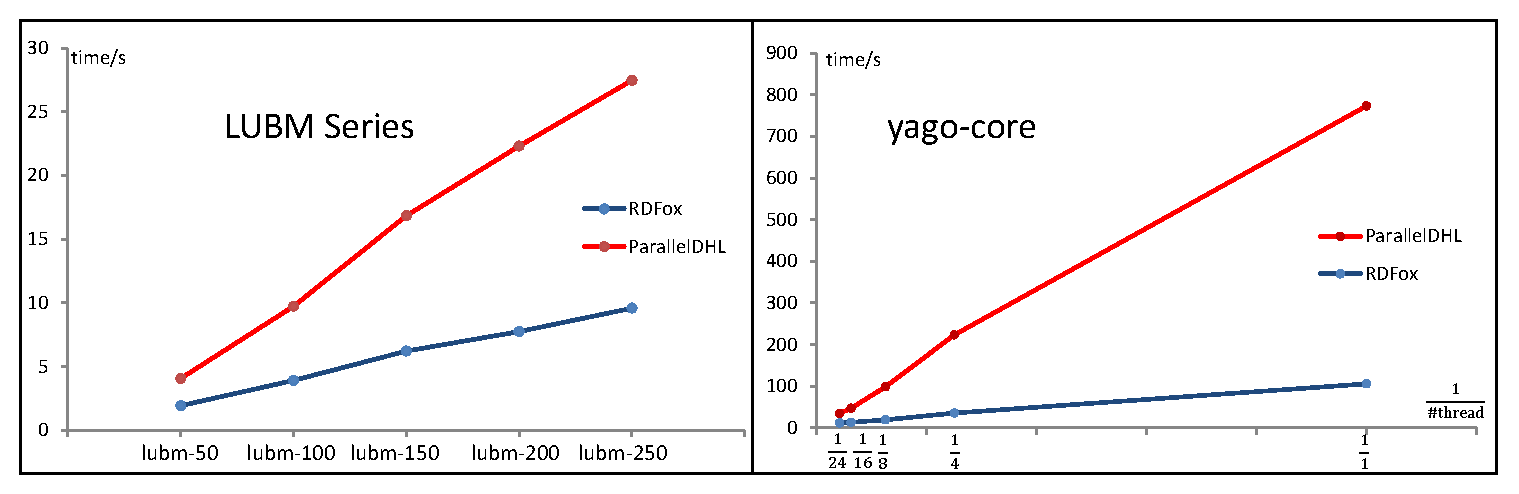
\includegraphics[width=1\textwidth]{fig-reasoningtime.eps}
\caption{(left) the reasoning times over the LUBM ontologies; (right) the reasoning times over yago-core.}
\label{fig:reasoningtime}
\end{center}
\end{figure}

From Table~\ref{tab:result}, we can see that for lubm-50 these two systems perform equally well.
For the other ontologies, ParallelDHL is comparable to RDFox with several threads being allocated.
For lubm-250 and yago-core, ParallelDHL delays obviously under only one thread.
The reason is that the computation of the relation $S_{\textit{\!\tiny rch}}$ occupies a large amount of time. When
four and more threads are allocated, ParallelDHL has a better efficiency.
Although ParallelDHL is not such optimized as RDFox, it also shows the scalability.
From the two line graphs in Figure~\ref{fig:reasoningtime},
we can see a linear trend of the reasoning times of both RDFox and ParallelDHL.
This also indicates that ParallelDHL will finish the materialization tasks on the test ontologies
in a shorter period of time with more threads being allocated.

\subsection{The Experiments on The Depths of Materialization Graphs}

From the complexity analysis for Algorithm~$\mathsf{A}_{bsc}$ (see Section~\ref{sec:alg-bsc}),
we have that the computing time of
Algorithm~$\mathsf{A}_{bsc}$ depends on the sizes of the input ontologies and the
numbers of iterations of \ref{alg1:updateG},
which equals to the depth of the target materialization graph (in the following,
we use the notion \emph{MG-depth} for short).
Thus, the MG-depth also determines the computing time of
Algorithm~$\mathsf{A}_{bsc}$ in theory.
This conclusion also applies to Algorithm~$\mathsf{A}_{opt}$ and Algorithm~$\mathsf{A}_{\texttt{prc}}$
based on the analysis in Section~\ref{sec:opt} and Section~\ref{sec:practicalAlg} respectively.
In this part, we examine the effects of MG-depths.

\begin{figure}[htbp]
\begin{center}
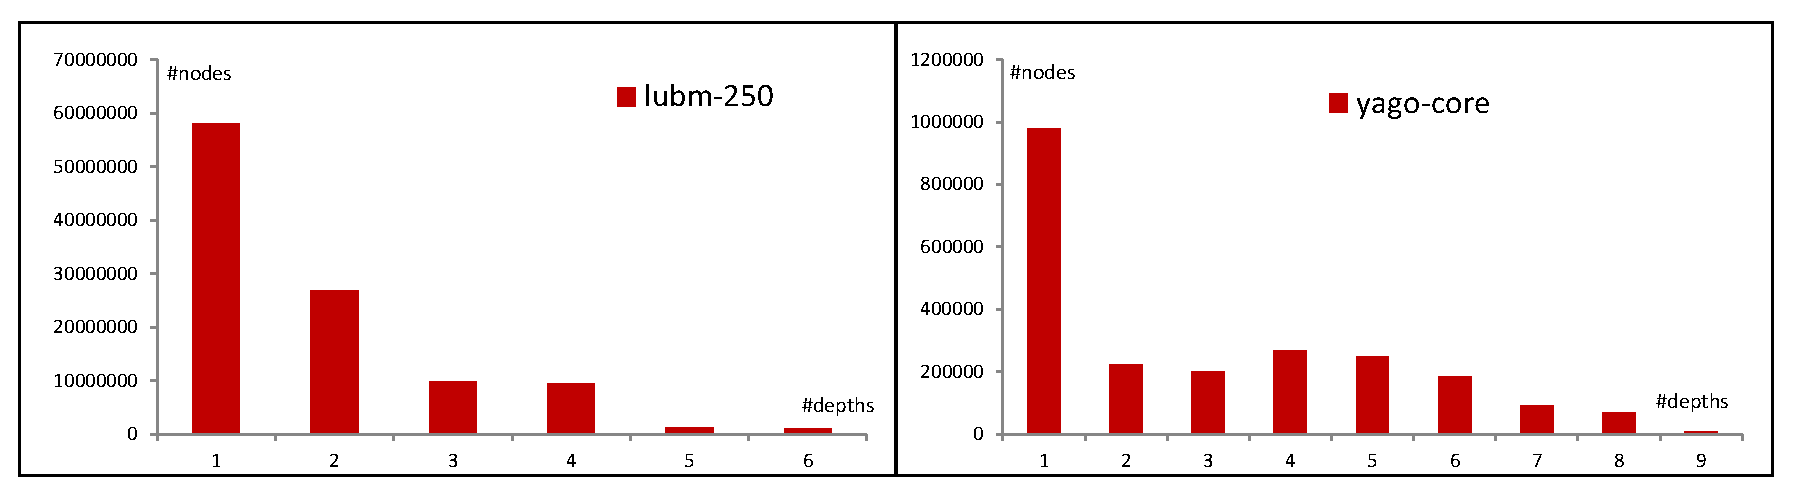
\includegraphics[width=1\textwidth]{fig-graphdepth.eps}
\caption{The numbers of nodes in different depths of lubm-250 (left) and yago-core (right).}
\label{fig:graphdepth}
\end{center}
\end{figure}

\textbf{The MG-Depths of LUBM and YAGO.}
For the five generated LUBM datasets and the yago-core ontology, we record the MG-depth
for each ontology and the number of nodes in different depths.
We have that all of the LUBM datasets have the MG-depth of 6,
and the MG-depth of the yago-core ontology is 9.
We use the histograms to graphically display the detailed data of lubm-250 and yago-core in Figure~\ref{fig:graphdepth},
where for each of the two histograms
the abscissa records the depths from the bottom of a materialization graph to the top,
the histograms denote the amount of nodes in each depth.
%
From the above results, we can find that the MG-depths are far less than
the sizes of the input ontologies. In these cases, the input ontology size
turns out to be the dominant factor for the reasoning efficiency.
This is also shown in Figure~\ref{fig:reasoningtime}(left) for the LUBM datasets,
where the reasoning times grow proportionally with the increasing of the number
of universities.
%
Thus, it is hard for us to use the above experiments to
observe the effects of MG-depths.

\textbf{Generating Ontologies of Different MG-Depths}.
In order to examine the effects of MG-depths, we consider modifying the core LUBM ontology
such that ontologies of different MG-depths can be obtained.
Inspired by Example~\ref{exp:simpleC},
we add to the core LUBM ontology the following three axioms to
describe the reference relationships among articles:
\begin{enumerate}[leftmargin=8ex,label=($\beta_{\arabic*}$),ref=$\beta_{\arabic*}$]
  \item $\exists\texttt{referTo}.\texttt{CollegeArtical}\sqsubseteq\texttt{CollegeConference}$\label{ptu:a1}
  \item $\exists\texttt{cite}.\top\sqsubseteq\texttt{CollegeSession}$\label{ptu:a2}
  \item $\texttt{CollegeConference}\sqcap\texttt{CollegeSession}\sqsubseteq\texttt{CollegeArtical}$\label{ptu:a3}
\end{enumerate}
where axiom~\ref{ptu:a1}, axiom~\ref{ptu:a2} and axiom~\ref{ptu:a3} give the
statements respectively: any article referring to a college article is published in a
college conference, any article having citations is published in a college session,
any article published in both of a college conference and a college session is
a college article.

We name the above new ontology PTU.
Based on the new added axioms in PTU, we further modify the ontology-generator
of LUBM such that a \emph{reference chain} of articles can be generated as follows:
$\texttt{referTo}(\texttt{a}_i,\texttt{a}_{i+1})$ and
$\texttt{cite}(\texttt{a}_i,\texttt{a}_{i+1})$ ($i\in\{0,1,2,...\}$),
where $\texttt{a}_i$ denotes an article instance.
As discussed in Section~\ref{sec:lubm-yago},
the original core ontology of LUBM is tractable in parallel via
Skolemization. Further, it can be checked that the concepts in PTU
are all simple concepts. Thus, PTU belongs to the parallel tractability class.
For comparison, we create another core ontology, named NPTU, which
is not tractable in parallel. NPTU is almost the same as PTU except that
axiom~\ref{ptu:a2} in PTU is replaced by the following axiom:
\begin{enumerate}[leftmargin=8ex]
  \item[($\beta_4$)] $\exists\texttt{cite}.\texttt{CollegeArtical}\sqsubseteq\texttt{CollegeSession}$\label{nptu:a1}
\end{enumerate}
which describes that any article citing a college article is published in a
college session.
It can be checked that NPTU does not follow the simple-concept restriction
by referring to Example~\ref{exp:dhl}.

The two core ontologies, PTU and NPTU,
and the modified ontology-generator are available online.\footnote{https://github.com/quanzz/PT}
To reduce the effects of ontology sizes, we generate five datasets of
the similar sizes for PTU (resp., NPTU), denoted by
ptu-$4m$-$i$ (resp., nptu-$4m$-$i$), $i\in\{1,2,4,8,16\}$,
where $i$ is the number of article reference chains
and $4m$ denotes that 4 million articles are involved averagely in all of the reference chains.
The statistics of the these generated datasets are given in Table~\ref{tab:generated}.
We can check from Table~\ref{tab:generated} that the datasets ptu-$4m$-$i$ ($i\in\{1,2,4,8,16\}$)
have the close number of assertions while the MG-depths decrease proportionally. This is
similar to the datasets nptu-$4m$-$i$ ($i\in\{1,2,4,8,16\}$).

\begin{table}
\centering
\caption{The statistics of the generated datasets}
\begin{tabular}{|l|r|r|r|r|r|r|}
\hline
ontology&$\sharp$concept&$\sharp$role&$\sharp$individual&$\sharp$axiom&$\sharp$assertion&MG-depth\\
\hline
ptu-$4m$-1&\multirow{10}{*}{51}&\multirow{10}{*}{34}&\multirow{10}{*}{4,000,440}&\multirow{10}{*}{102}&8,000,839&8,000,799\\
ptu-$4m$-2&&&&&8,000,837&4,000,399\\
ptu-$4m$-4&&&&&8,000,835&2,000,199\\
ptu-$4m$-8&&&&&8,000,833&1,000,099\\
ptu-$4m$-16&&&&&8,000,831&500,049\\
nptu-$4m$-1&&&&&8,000,839&8,000,799\\
nptu-$4m$-2&&&&&8,000,837&4,000,399\\
nptu-$4m$-4&&&&&8,000,835&2,000,199\\
nptu-$4m$-8&&&&&8,000,833&1,000,099\\
nptu-$4m$-16&&&&&8,000,831&500,049\\
\hline
\end{tabular}
\label{tab:generated}
\end{table}

\textbf{Experimental Results and Analysis}.
We run RDFox and ParallelDHL on the generated datasets respectively. The detailed experimental results
can be found at the address.\footnote{https://github.com/quanzz/PT} We give Table~\ref{tab:speedup} to compare the reasoning times and
speedups\footnote{The speedup is computed by $\frac{T_1}{T_n}$ where $T_1$ is the computing time
under 1 thread and $T_n$ is the computing time under $n$ thread(s).}
of the two systems when handling nptu-$4m$-1 and ptu-$4m$-1.
We further give Figure~\ref{fig:diffdepths} and Figure~\ref{fig:diffthreads} to show the trends of
reasoning times. Specifically, the two line graphs of Figure~\ref{fig:diffdepths}
show the reasoning times of RDFox and ParallelDHL over
all the generated datasets with 24 threads being allocated;
in Figure~\ref{fig:diffthreads},
the abscissas of the two line graphs record the reciprocals of the numbers of threads, and
the ordinates record the reasoning times over nptu-$4m$-1 and ptu-$4m$-1 respectively.

\begin{figure}[htbp]
\begin{center}
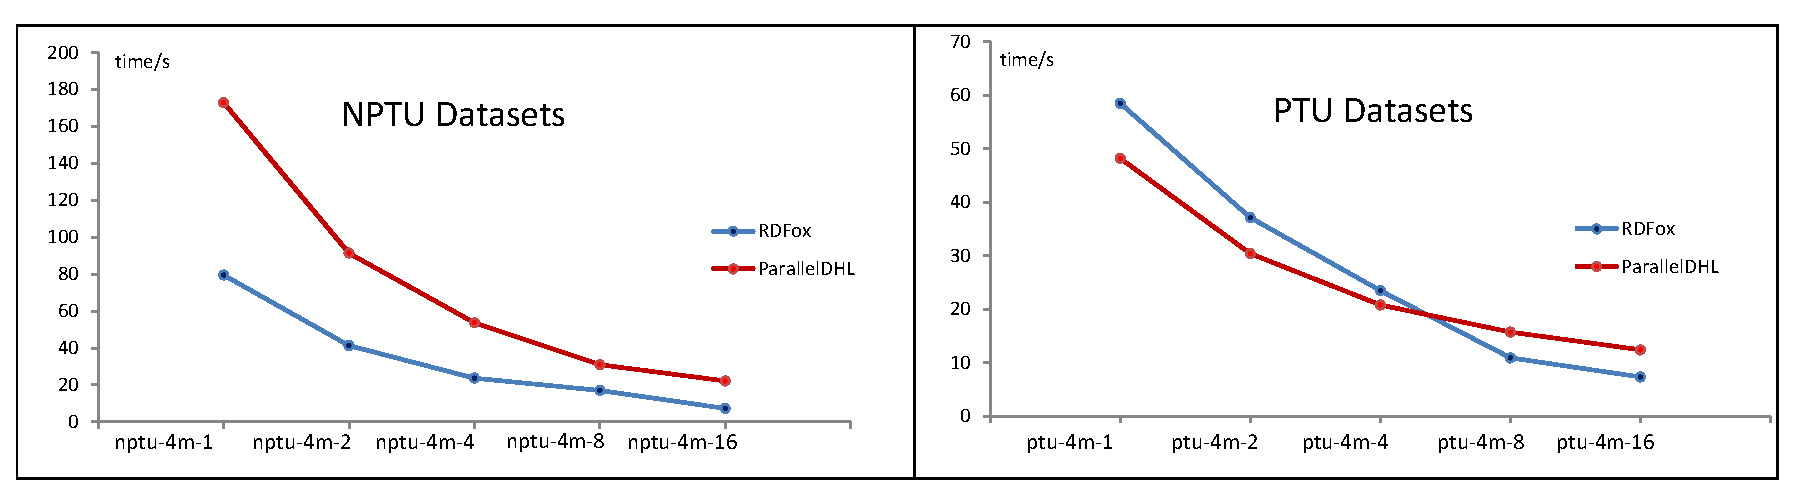
\includegraphics[width=1\textwidth]{fig-diff-depths.eps}
\caption{(left) the reasoning times over NPTU datasets; (right) the reasoning times over PTU datasets.}
\label{fig:diffdepths}
\end{center}
\end{figure}

It can be shown from Figure~\ref{fig:diffdepths} that MG-depths indeed determine
the reasoning times.
For the five datasets, nptu-$4m$-$i$, where $i\in\{1,2,4,8,16\}$, the experimental
results show an obvious downtrend of the reasoning times with the declining of the MG-depths for
both of RDFox and ParallelDHL (see Figure~\ref{fig:diffdepths}(left)).
The downtrend of reasoning times also exists
when handling the datasets ptu-$4m$-$i$ (see Figure~\ref{fig:diffdepths}(right)), where $i\in\{1,2,4,8,16\}$.
Although the NPTU and PTU datasets are unrealistic in practice, these experiments indeed
verify that MG-depths determines the reasoning time in parallel
considering that the input ontology sizes are close.

\begin{table}
\centering
\caption{The reasoning-times (seconds) and speedups}
\begin{tabular}{|l|r|r|r|r|r|}
\hline
&\small$\sharp$thread&nptu-$4m$-1&speedup&ptu-$4m$-1&speedup\\
\hline
\multirow{5}{*}{ \textbf{RDFox}}&1&50.95&1&20.55&1\\
                                &4&72.42&0.7&56.48&0.36\\
                                &8&74.43&0.68&54.52&0.38\\
                                &16&74.23&0.69&60.98&0.34\\
                                &24&79.46&0.64&58.47&0.35\\
\hline
\multirow{5}{*}{ \small{\textbf{ParallelDHL}}}&1&135.79&1&252.13&1\\
                                &4&142.34&0.95&147.2&1.71\\
                                &8&145.04&0.93&102.83&2.45\\
                                &16&156.05&0.87&56.48&4.46\\
                                &24&172.81&078&48.19&5.23\\
\hline
\end{tabular}
\label{tab:speedup}
\end{table}

We now discuss the issue of parallel tractability based on the experimental
results of nptu-$4m$-1 and ptu-$4m$-1.
From Figure~\ref{fig:diffthreads}(left),
we can see that for both of RDFox and ParallelDHL the reasoning efficiency are not
improved when several threads are allocated. On the contrary, with less than 24 threads are allocated,
the materialization costs less time. In detail,
the reasoning time of RDFox under 24 threads
is 79.46 seconds, while it costs 50.95 seconds under only one thread.
Further, the speedups of RDFox stay below 1 under more than 1 threads (see Table~\ref{tab:speedup}).
This means that the reasoning times cannot reduced with more than 1 threads being
allocated.
This ``abnormal" situation also happens for ParallelDHL.
This situation is caused by the issue of path twisting.
The NPTU ontology does not follow the simple-concept restriction since
concepts \texttt{CollegeConference} and \texttt{CollegeSession} are not simple.
The materialization over nptu-$4m$-$i$ ($i\in\{1,2,4,8,16\}$) suffers from the issue
of path twisting which is similar to the case in Example~\ref{exp:dhl}.
Specifically, the axioms of the form \texttt{CollegeArtical}$(a_i)$ are
the joint nodes in the twisted path.
According to the analysis for Example~\ref{exp:dhl}, parallel computation can hardly
handle this case. Moreover, the dataset nptu-$4m$-1 has only one
article reference chain. This means that all
the axioms of the form \texttt{CollegeArtical}$(a_i)$ actually
appear in one path of the target materialization graph.
Thus, they depends on each other and cannot be derived in parallel.
On the other hand, the working mechanism of RDFox and ParallelDHL is based on
a thread pool, where several threads are maintained and scheduled.
The maintaining and scheduling of the thread pool also produce
overheads, in particular, when the parallel computation
cannot improve the total efficiency.
This is why the materialization over nptu-$4m$-1 under one
thread has a better performance.

\begin{figure}[htbp]
\begin{center}
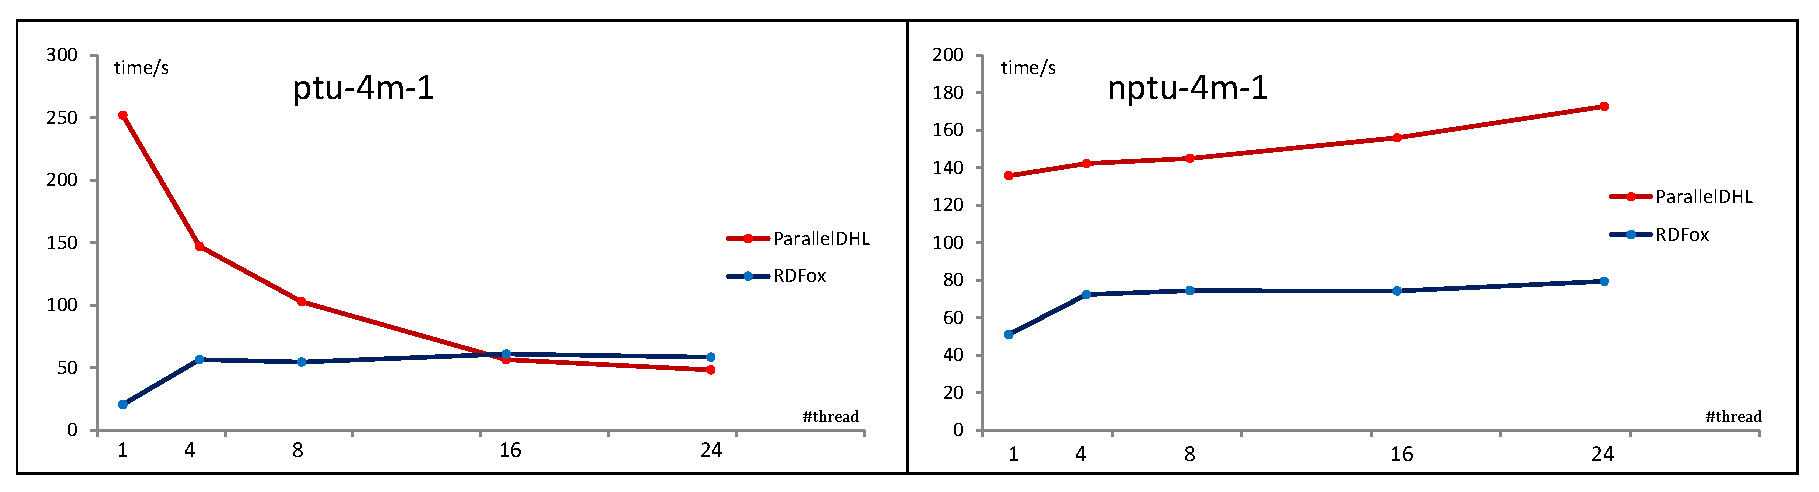
\includegraphics[width=1\textwidth]{fig-diff-threads.eps}
\caption{(left) the reasoning times over nptu-$4m$-1; (right) the reasoning times over ptu-$4m$-1.}
\label{fig:diffthreads}
\end{center}
\end{figure}

For the dataset ptu-$4m$-1, the trends of reasoning times are different
between RDFox and ParallelDHL.
Similarly to the case of handling nptu-$4m$-1,
the acceleration effect for RDFox is not outstanding
over ptu-$4m$-1. The speedups under different numbers of threads stay around 1 (see Table~\ref{tab:speedup}).
This means that reasoning times are not reduced with the increasing of the number of threads.
The results of ParallelDHL show a better acceleration effect.
From Table~\ref{tab:speedup}, with only one thread being allocated, ParallelDHL finishes
the materialization on ptu-$4m$-1 in 135.79 seconds. When four and more threads
are allocated, the reasoning performance is obviously improved.
The maximal speedup reaches up to 5.23 under 24 threads.
Specially, under more than 16 threads, ParallelDHL
costs less time to finish the materialization with compared to RDFox.
From Figure~\ref{fig:diffthreads}(right), there is an obvious downtrend of the reasoning times
from one thread to 24 threads.
The main reason of the difference between RDFox and ParallelDHL
lays in that the PTU ontology is tractable in parallel and ParallelDHL
is optimized based on the SWD paths. The PTU ontology follows the
simple-concept restriction. Thus, there is no twisting path in
the materialization graph of ptu-$4m$-1 although all articles are involved
in one reference chain. This allows that the relation $S_{\textit{\!\tiny rch}}$ can be computed
only once in the second iteration of \ref{alg3:updateG} of Algorithm~$\mathsf{A}_{\text{prc}}$
when handling ptu-$4m$-1 (referring to the analysis for Example~\ref{exp:simpleC}).
It can also be checked that all the axioms of the form \texttt{CollegeArtical}$(a_i)$ occur in
an SWD path. Thus, the optimization based on SWD paths work when handling ptu-$4m$-1.
For RDFox, since it is not optimized specially for this case, it performs the task of
materialization over ptu-$4m$-1 similarly to that over nptu-$4m$-1;
specifically, the axioms of the form \texttt{CollegeArtical}$(a_i)$ are derived sequentially.
From Figure~\ref{fig:diffdepths}(right), we can see that the optimization used in ParallelDHL
also leads to a better performance compared to
RDFox when handling ptu-$4m$-1, ptu-$4m$-2 and ptu-$4m$-4 under 24 threads.

%%% Local Variables:
%%% mode: latex
%%% TeX-master: "parallel-tractability-J"
%%% End:


\section{Related Work}
\label{sec:related}

The parallel reasoner RDFox \cite{MotikNPHO14} is used to evaluate our implementation. RDFox is a state-of-the-art system that handles reasoning on datalog rewritable ontology languages. Algorithm~$\mathsf{A}_{bsc}$ proposed in Section~\ref{sec:ptclass}, is similar to the main algorithm of RDFox (see \cite{MotikNPHO14}, Sections~3 and 4). The main difference is that a group of rule instantiations is handled by one processor (namely a thread) in RDFox, while in Algorithm~$\mathsf{A}_{bsc}$, each rule instantiation is assigned to a unique processor. Thus, in theory, the materialization of the datalog program in Example~\ref{exp:mg} is serial in RDFox {\color{red}The example has two rules. Why can they not be parallelized in RDFox?}. ItThe experiments also show that parallelism does not lead to a remarkable improvement for RDFox for the ontology series not in $\mathcal{D}_{\textit{\text{dhl}}(\circ)}$. We use Algorithm~$\mathsf{A}_{opt}$ to show that the ontology in Example~\ref{exp:mg} is also tractable in parallel. Our implementation ParallelDHL, which is based on Algorithm~$\mathsf{A}_{prc}$, also shows a better performance than RDFox when handling the test ontologies that belong to $\mathcal{D}_{\textit{\text{dhl}}(\circ)}$.

There is work that studies parallel reasoning in RDFS and OWL. The current methods mainly focus on optimizing reasoning algorithms from different aspects. \citet{GoodmanJMAAH11} propose a new kind of encoding method for RDF triples to achieve a high performance. This method can significantly yield a throughput improvement and optimize parallel RDF reasoning and query answering. \citet{PetersSZ15} use the RETE algorithm to accelerate rule matching for RDFS reasoning. \citet{SubercazeGCL16} propose a more efficient storage technique and optimize the join operations in parallel reasoning. The issue of balance distribution of parallel tasks is also studied \cite{SomaP08,WeaverH09}. Two approaches are explored, i.e., \emph{rule partitioning} (allocating parallel tasks to different processors based on rules) and \emph{data partitioning} (allocating parallel tasks based on data). The evaluation results indicate that the efficiency of balance distribution varies with respect to different datasets. On the other hand, parallel reasoning is also implemented for OWL fragments, e.g., OWL~RL \cite{KolovskiWE10}, OWL~EL \cite{KazakovKS14}, OWL~QL \cite{LemboSS13}, and even highly expressive languages \cite{SteigmillerLG14,LiebigM07,SchlichtS08,WuH12}. In current work, several techniques are proposed to adapt parallel computation to OWL reasoning tasks. A kind of graph-based method is discussed by \citet{LemboSS13} to enhance OWL~QL classification.  Several pruning techniques are proposed to optimize the Tableaux algorithm \cite{LiebigM07,SchlichtS08,WuH12}. The \emph{lock-free technique} is applied by \citet{KazakovKS14} and \citet{SteigmillerLG14}.

Another line of optimizing parallel reasoning is to utilize high-performance computing platforms. For in-memory platforms, different supercomputers such as Cray XMT or Yahoo S4 have early on been used in parallel RDF reasoning \cite{Hoeksema2011,GoodmanJMAAH11}. \citet{HeinoP12} report on their work on RDFS reasoning based on massively parallel GPU hardware. Distributed parallel platforms such as MapReduce and Peer-to-Peer networks are also used for RDFS reasoning. The representative systems are WebPIE \cite{UrbaniKMHB12}, Marvin \cite{oren2009marvin} and SAOR \cite{HoganHP09}. Different techniques are discussed in this work to tackle the special problems in distributed computing. However, to study the issue of parallel tractability on distributed platforms,  more issues have to be discussed, e.g., \emph{network structures} and \emph{communications}. This is not the focus in this paper.

Different from the above work, the purpose of this paper is to study the issue of the parallel tractability of materialization from the perspective of data. The results given in this paper guarantee the parallel tractability theoretically, regardless of what optimization techniques and platforms as discussed above are used.




%%% Local Variables:
%%% mode: latex
%%% TeX-master: "parallel-tractability-J"
%%% End:


\section{Conclusions}
\label{sec:conclusion}

In this paper, we studied the problem of parallel tractability of
materialization on the datalog rewritable ontologies.
To identify the parallelly tractable classes,
we proposed two NC algorithms, Algorithm~$\mathsf{A}_{bsc}^\psi$
and Algorithm~$\mathsf{A}_{opt}^\psi$, that perform materialization on
datalog rewritable ontology languages.
Based on these algorithms, we identified the corresponding
parallelly tractable datalog program (\texttt{PTD}) classes such that materialization
on the datalog programs in these classes is in the complexity class NC.
We further studied two specific ontology languages, DL-Lite and DHL (including one of its extension).
We showed that any ontology expressed in DL-Lite$_{core}$ or DL-Lite$_{\mathcal{R}}$ is parallelly tractable.
For DHL and DHL($\circ$), we proposed two restrictions such that materialization is parallelly tractable.

We verified the usefulness of our theoretical techniques in two ways. On the one hand,
we analyzed different kinds of datasets,
including well-known benchmarks, real-world ontologies and a famous dataset YAGO.
Our analysis showed that many real ontologies belong to
the parallelly tractable class $\mathcal{D}_{\textit{\text{dhl}}}$
or $\mathcal{D}_{\textit{\text{dhl}}(\circ)}$. The
developers and users can also refer to $\mathcal{D}_{\textit{\text{dhl}}}$
and $\mathcal{D}_{\textit{\text{dhl}}(\circ)}$
to create large-scale ontologies for which parallel tractability
is theoretically guaranteed. On the other hand,
we used an optimization strategy based on SWD paths
to give a practical algorithm variant Algorithm~$\mathsf{A}_{prc}$, which can
also be restricted to an NC version, and can be implemented for practice.
We implemented a system based on Algorithm~$\mathsf{A}_{prc}$ and compared it to
the state-of-the-art reasoner RDFox.
The experimental results showed that the optimization proposed in this paper results
in a better performance on parallelly tractable ontologies compared with RDFox.

In the future work, we will extend our work in two lines.
One line is a further study of the parallel tractability of
other expressive ontology languages, in addition to
datalog rewritable ones. Since different expressive OWL languages
have different syntaxes and higher reasoning complexities than \texttt{PTime}-complete, we need to
explore more restrictions that are practical and make materialization
parallelly tractable. Another line of the future work is to
study how to further apply the
results in practice.
One idea is to apply the technique of SWD paths to enhance other reasoning-based tasks,
like ontology classification, ontology debugging and query answering.




%%% Local Variables:
%%% mode: latex
%%% TeX-master: "parallel-tractability-J"
%%% End:


\section*{Acknowledgments}

This work was partially supported by NSFC
grant 61672153 and the 863 program under Grant
2015AA015406.

%\bibliographystyle{elsarticle-num}
\bibliographystyle{elsarticle-num-names}
\bibliography{reference}

\clearpage

\section*{Appendix}

\appendix

\section{Proof of Lemma~\ref{lemma:a1}}

\textbf{Lemma~\ref{lemma:a1}}
\emph{Given a datalog program $P=\langle R, \textbf{I}\rangle$, we have
(1) $\mathsf{A}_{\text{bsc}}$ halts and returns a materialization graph $\mathcal{G}$ of $P$;
(2) $\mathcal{G}$ has the the minimum depth among all the materialization graphs of $P$.}\\

\noindent\emph{Proof}:
(1) First, whenever a processor $p$ adds a new node $v$ to $\mathcal{G}$, it has to first
check whether $v$ has already been in $\mathcal{G}$ and does nothing if $v$ is in $\mathcal{G}$.
Thus $\mathcal{G}$ turns out to be an acyclic graph.
Second, to show $\mathcal{G}$ is a
complete materialization graph, we perform an induction on $T_R^{\omega}(\textbf{I})$.
Specifically, all the facts in $T_R^{0}(\textbf{I})$ have to be in $\mathcal{G}$ by \ref{alg1:addFacts}
of $\mathsf{A}_{\text{bsc}}$.
For $i>0$, suppose that the ground atoms in $T_R^{i}(\textbf{I})$ are in $\mathcal{G}$.
It can be checked that the atoms in $T_R^{i+1}(\textbf{I})$ have to be
added to $\mathcal{G}$, since whenever a new node is derived from $T_R^{i}(\textbf{I})$,
there has to be a processor that would add it to $\mathcal{G}$.

(2) The \emph{stage} (see the related contents in Section~2.3) of $P$ is the lower bound of the depth
of all materialization graphs. One can further check that, for the materialization graph $\mathcal{G}$
constructed by $\mathsf{A}_{\text{bsc}}$, its depth is equal to the stage based on the induction above.
Thus, $\mathcal{G}$ has the minimal depth among all the materialization graphs of $P$. \hfill$\Box$

\section{Proof of Theorem~\ref{theorem:a1}}

\textbf{Theorem~\ref{theorem:a1}}
\emph{For any datalog program $P=\langle R, \textbf{I}\rangle$, $P\in\mathcal{D}_{\mathsf{A}_{\text{bsc}}^{\psi}}$ iff
$P$ has a materialization graph whose depth is upper-bounded by $\psi(|\textbf{I}|)$.}\\

\noindent\emph{Proof:} We first prove that the number of iterations of \ref{alg1:updateG}
is actually the depth of the constructed materialization graph.
We define the depths of nodes iteratively as follows:
for each of the original node $v$, \texttt{depth}($v$)=0;
for each implicit node $v'$ whose parents are $v_1,...,v_i$, \texttt{depth}($v'$)=$\max$$\{$ \texttt{depth}($v_1$), ..., \texttt{depth}($v_i$) $\}+1$.
By performing an induction on the number of iterations of \ref{alg1:updateG},
one can check that an implicit node $v'$ has to be added to $\mathcal{G}$ in the $n^{th}$ iteration
where $n$=\texttt{depth}($v'$).
Further, \texttt{depth}($\mathcal{G}$)=$\max$$\{$\texttt{depth}($v_i$)$|v_i$ is in $\mathcal{G}\}$.
We then have that the number of iterations of \ref{alg1:updateG} is \texttt{depth}($\mathcal{G}$).

($\Rightarrow$) $P\in\mathcal{D}_{\mathsf{A}_{\text{bsc}}^{\psi}}$ means that $\mathsf{A}_{\text{bsc}}^{\psi}$ can return
a materialization graph $\mathcal{G}$ of $P$.
Recall that the number of iterations of \ref{alg1:updateG} is bounded by $\psi(|\textbf{I}|)$.
Thus \texttt{depth}($\mathcal{G}$) is also bounded by $\psi(|\textbf{I}|)$.

($\Leftarrow$) Suppose $P$ has a materialization graph $\mathcal{G}$ whose depth
is upper-bounded by $\psi(|\textbf{I}|)$.
If $\mathcal{G}$ has the minimal depth among other materialization graphs of $P$,
the number of iterations of \ref{alg1:updateG} is also \texttt{depth}($\mathcal{G}$) (Lemma~\ref{lemma:a1})
and, thus, upper-bounded by $\psi(|\textbf{I}|)$.
If $\mathsf{A}_{\text{bsc}}$ dose not return $\mathcal{G}$, then the returned graph $\mathcal{G}'$
should have a smaller depth compared with $\mathcal{G}$.
In this case, this conclusion still holds.\hfill$\Box$

\section{Proof of Lemma~\ref{lemma:a3}}

\textbf{Lemma~\ref{lemma:a3}}
\emph{Given a datalog program $P=\langle R, \textbf{I}\rangle$,
$\mathsf{A}_{\text{opt}}$ halts and outputs a materialization graph
$\mathcal{G}$ of $P$.}\\

\noindent\emph{Proof}: We prove the lemma in two stages:
(1) the graph $\mathcal{G}$ returned by $\mathsf{A}_{\text{opt}}$ is a materialization graph;
(2) $\mathcal{G}$ is a complete materialization graph.
We first show that (1) holds by an induction on the iterations of \ref{alg3:updateG} of $\mathsf{A}_{\text{opt}}$.

\emph{Base case}. Initially, $\mathcal{G}$ only contains all the original nodes.
In this case, $\mathcal{G}$ is obviously a materialization graph.

\emph{Inductive case}.
According to the induction hypothesis, the partial graph constructed after
the $i^{th}$ ($i>1$) iteration is a materialization graph, denoted by $\mathcal{G}^{i}$.
We have to show that the partial graph constructed after the $(i+1)^{th}$ iteration is
also a materialization graph, denoted by $\mathcal{G}^{i+1}$.
The partial graph $\mathcal{G}^{i+1}$ is updated in $\mathsf{A}_{\text{opt}}$ by performing Step $(\textbf{\romannumeral3})$
of Algorithm~$\mathsf{OPT}$.
Suppose that \texttt{rch}$(B_k,H)\in S_{\textit{\!\tiny rch}}$ is checked.
It corresponds to the rule instantiation $B_1,..,B_k,..,B_n\rightarrow H$.
Algorithm~$\mathsf{OPT}$ next checks that there exists a node $B'$ such that
\texttt{rch}$(B',B_k)\in S^*_{\!\tiny rch}$
and $B'$ is in $\mathcal{G}$. This means that $B_k$ and $H$ are derivable.
The algorithm then adds new nodes $B_k$ and $H$ to $\mathcal{G}^{i}$
according to three cases.
(1) If $H$ is not in $\mathcal{G}^{i}$ while $B_k$ is in $\mathcal{G}^{i}$,
then $H$ is added to $\mathcal{G}^{i+1}$, and the edges $e(B_1, H),...,e(B_n, H)$ are created.
(2) If neither of $H$ and $B_k$ is in $\mathcal{G}^{i}$,
then $H$ and $B_k$ are added to $\mathcal{G}^{i+1}$, and the edges $e(B_1, H),...,e(B_n, H)$ are also created.
In the above two cases, $H$ is a new node. Thus,
$\mathcal{G}^{i+1}$ is acyclic.
(3) If $H$ is in $\mathcal{G}^{i}$ and $H$ has no parent,
$B_k$ is added to $\mathcal{G}^{i+1}$, and the edges $e(B_1, H),...,e(B_n, H)$ are also created.
For the case that $H$ is in $\mathcal{G}^{i}$ and $H$ has parents,
the algorithm does nothing.
Thus, $\mathcal{G}^{i+1}$ is acyclic and satisfies the definition of materialization graph.

To show that (2) holds, we use the same method as in the proof of Lemma~\ref{lemma:a1}.
We want to show that all the ground atoms in $T_R^{i+1}(\textbf{I})$ have to be added to $\mathcal{G}$,
with the induction hypothesis that the ground atoms in $T_R^{i}(\textbf{I})$ are in $\mathcal{G}$.
Suppose the ground atoms in $T_R^{i}(\textbf{I})$ have been added to $\mathcal{G}$ by
performing $\mathsf{A}_{\text{opt}}$.
For each atom $\alpha$ in $T_R^{i+1}(\textbf{I})$, $\alpha$ actually has a special SWD path
of length~$1$. This is because all parents of $\alpha$ have been in $\mathcal{G}$.
According to the optimization strategy, $\alpha$ has to be added to $\mathcal{G}$ by applying \ref{alg3:updateG}
of $\mathsf{A}_{\text{opt}}$.\hfill$\Box$


\section{Proof of Lemma~\ref{lemma:dllite}}

\textbf{Lemma~\ref{lemma:dllite}}
\emph{For any DL-Lite$_{\text{core}}$ or DL-Lite$_\mathcal{R}$ ontology $\mathcal{O}$, there exists a materialization graph $\mathcal{G}$ such that
each atom of the form $A(x)$ ($A\neq\bot$) or $R(x,y)$ in $\mathcal{G}$ has an SWD path.}\\

\noindent\emph{Proof}: We first prove the lemma by an induction on applications of
the datalog rules corresponding to DL-Lite$_\mathcal{R}$ axioms.\\

\emph{Base case}. For each of the original node $v$ of the form $A(x)$ ($A\neq\bot$) or $R(x,y)$,
$v$ has a special SWD path with $v$ as the unique node. This conclusion holds
for any materialization graph.

\emph{Inductive cases}. For each datalog rule of the form `$B_1,...,B_n\rightarrow H$'
that is rewritten from some DL-Lite$_\mathcal{R}$ axiom, we have the induction hypothesis
that $B_1,...,B_n$ have SWD paths.
We are left to prove that $H$ has an SWD path as well
in all materialization graphs of $\mathcal{O}$.

If $H$ is in the form of $A(x)$ ($A\neq\bot$), it may be derived by
applying (T1) and (T3). Thus, we conduct the induction by
distinguishing these two cases as follows:

\begin{enumerate}[leftmargin=12ex,label=Case~1.\arabic*]
\item $B\sqsubseteq A$. According to the induction hypothesis,
node $B(x)$ has an SWD path, denoted by $(v_1,...,v_n,B(x))$.
We have that, in some materialization graph, node $A(x)$
has an SWD path of the form $(v_1,...,v_n,B(x),A(x))$.

\item $\exists R\sqsubseteq A$. Node $R(x,y)$ has an SWD path,
denoted by $(v_1,...,v_n,R(x,y))$,
according to the induction hypothesis.
It is obvious that node $A(x)$
has an SWD path of the form $(v_1,...,v_n,B(x),R(x,y))$
in some materialization graph.
\end{enumerate}

Since node $A(x)$ can only be derived in either Case~1.1
or Case~1.2, we have that
node $A(x)$ has an SWD path in all materialization graphs of $\mathcal{O}$.

It is similar to prove the case where $H$ is in the form of $R(x,y)$.
Since node $R(x,y)$ may be derived by
applying (R1) and (R2), we discuss these two cases.

\begin{enumerate}[leftmargin=12ex,label=Case~2.\arabic*]
\item $S\sqsubseteq R$. According to the induction hypothesis,
node $S(x,y)$ has an SWD path, denoted by $(v_1,...,v_n,S(x,y))$.
Obviously, node $R(x,y)$
has an SWD path of the form $(v_1,...,v_n,S(x,y),R(x,y))$
in some materialization graph.

\item $S\sqsubseteq R^-$. This case is similar to
the above case.
\end{enumerate}

For both Case~2.1 and Case~2.2, node $R(x,y)$ has an SWD path. Thus,
node $R(x,y)$ has an SWD path in all materialization graphs of $\mathcal{O}$.
We finish the proof for DL-Lite$_\mathcal{R}$. Since 
DL-Lite$_{\text{core}}$ is a subset of DL-Lite$_\mathcal{R}$
in terms of the expressivity, the above conclusion also applies
to DL-Lite$_{\text{core}}$.\hfill$\Box$


\section{Proof of Theorem~\ref{theorem:dl-lite}}

\textbf{Theorem~\ref{theorem:dl-lite}}
\emph{There exists a poly-logarithmically bounded function $\psi$ s.t.
$\mathcal{D}_{\textit{\text{dl-lite}}}\subseteq\mathcal{D}_{\mathsf{A}_{\text{opt}}^{\psi}}$.}\\

\noindent\emph{Proof}: this theorem can be easily proved based on Lemma~\ref{lemma:dllite}.
Specifically, for any DL-Lite$_{\text{core}}$ or DL-Lite$_\mathcal{R}$ ontology $\mathcal{O}$,
there always exists a poly-logarithmically bounded function $\psi$ such that
$\mathsf{A}_{\text{opt}}^{\psi}$ can handle the materialization of $\mathcal{O}$,
since in any materialization graph, each node has an SWD path.
More precisely, we can set that $\psi=2$.\hfill$\Box$


\section{Proof of Theorem~\ref{theorem:dhl}}

\textbf{Theorem~\ref{theorem:dhl}}
\emph{There exists a poly-logarithmically bounded function $\psi$ s.t.
$\mathcal{D}_{\textit{\text{dhl}}}\subseteq\mathcal{D}_{\mathsf{A}_{\text{opt}}^{\psi}}$.}\\

\noindent\emph{Proof}: observe that, for a datalog program that is transformed from a DHL ontology,
a rule with a binary atom as its head can only be either of the form (R1), (R2) or (R3).
This also indicates that, the materialization of a DHL
ontology can be separated into two stages: in the first stage (Stage~1), all the rules
of the forms (R1-R3) are exhaustively applied; the consequences of the first stage
also serve as the facts in the second stage (Stage~2). The rules of the forms (T1-T3)
are then applied in Stage~2.
It is obvious that, if both of Stage~1 and Stage~2 can be handled
by performing $\mathsf{A}_{\text{opt}}^\psi$ for some poly-logarithmical function $\psi$, then
the whole materialization can be handled by $\mathsf{A}_{\text{opt}}^\psi$.
In what follows, we investigate the above two stages respectively, and show that,
for any datalog program in $\mathcal{D}_{\textit{\text{dhl}}}$,
such a poly-logarithmical function $\psi$ exists.

In Stage~1, the rules of the forms (R1-R3)
are applied to add new nodes to the constructed materialization graph.
We can observe that, rule (R3) is used for computation of transitive roles.
As mentioned before, there exists an NC algorithm for transitivity computation.
Inspired by this, we can prove that \emph{$\mathsf{A}_{\text{opt}}^\psi$
handles Stage~1 for some poly-logarithmical function $\psi$}.
The proof of this result can be shown by separately considering non-transitive roles and
the roles that are transitive or influenced by transitive roles.
Specifically, we say that role $R$ is \emph{transitively influenced} (TI)
if (1) $R\circ R\sqsubseteq R\in\mathcal{R}$; or
(2) there exists a TI role $R'$ such that $R'\sqsubseteq_*R$ or $R'\sqsubseteq_*R^-$.
We say that a role is an NTI (non-transitively influenced) role if it is not a TI role.
We further define a set $\delta_R$ for each role $R\in\textbf{R}$ as follows:

\begin{definition}\label{def:deltaRdhl}
For each $R\in\textbf{R}$, let $\delta_R$ be the set of all assertions as follows:
\begin{enumerate}[leftmargin=4ex,label=\arabic*.]
\item for each $R(a,b)\in\mathcal{A}$;
\item $R(a,b)$, for each $R'(a,b)\in\mathcal{A}$ and $R'\sqsubseteq_{*}R$;
\item $R(a,b)$, for each $R'(b,a)\in\mathcal{A}$ and $R'\sqsubseteq_{*}R^-$.
\end{enumerate}
\end{definition}

Let $\delta^*_R$ be the transitive closure of $\delta_R$ where $R$ is a transitive role.
We then have the following lemma.

\begin{lemma}\label{lemma:ti}
$P\models R(a,b)$ implies: (1) if $R$ is an NTI role, $R(a,b)\in\delta_R$;
(2) if $R$ is a transitive role, $R(a,b)\in\delta^*_{R}$;
(3) if $R$ is a TI role, then $R(a,b)\in\delta_R$, or there exists a transitive
role $R'$ such that $R'\sqsubseteq_* R$ and $R'(a,b)\in\delta^*_{R'}$.
\end{lemma}

Note that, for all roles $R$, $\delta_R$ can be computed by only applying (R1) and (R2).
In this sense, Lemma~\ref{lemma:ti} also indicates that:
(1) for each implicit node $R(a,b)$ where $R$ is an NTI role,
it can be added to a materialization graph by only applying (R1) and (R2);
(2) for each transitive role $R$, all implicit nodes of the form $R(a,b)$ are in the transitive closure $\delta^*_{R}$,
which can be computed by an NC algorithm on $\delta_{R}$;
(3) for each role $R$ that is a TI role but not a transitive role,
one can further perform (R1) and (R2) iteratively based on all transitive closures $\delta^*_{R'}$
where $R'$ is a transitive role.
Since all nodes generated by only applying (R1) and (R2) have SWD paths,
the computations of (1) and (3) can be handled by $\mathsf{A}_{\text{opt}}^\psi$.
Further, transitive computation in part (2) can also be handled by $\mathsf{A}_{\text{opt}}^\psi$.
Thus, there exists a poly-logarithmical function $\psi$
such that $\mathsf{A}_{\text{opt}}^\psi$ handles Stage~1.

The results of Stage~1 serve as the facts of Stage~2. In other words, all binary atoms
are the original nodes in Stage~2. This also means that the rules of the forms (T1) and (T3)
generate nodes with SWD paths. Due to the simple-concept restriction, for each rule
instantiation $A_1(a),A_2(a)\rightarrow B(a)$, one of $A_1(a)$ and $A_2(a)$ always has an SWD path.
Thus, Stage~2 can be handled by $\mathsf{A}_{\text{opt}}$ in at most two iterations.
Based on the above analysis, this theorem holds.

We are now left to prove Lemma~\ref{lemma:ti}. We conduct the proof by an induction on
the derivation of $P=\langle R,\textbf{I}\rangle$. We distinguish inductive cases by different rules (R1-R3)
that are possibly applied to derive $R(a,b)$.

\emph{Basic case}. If $R(a,b)\in\textbf{I}$, $R(a,b)\in\delta_{R}$. In this case,
regardless of that $R$ is a TI or an NTI role, all of (1), (2) and (3) hold.

\emph{Inductive case}. We first study the case where $R$ is an NTI role.

\begin{enumerate}[leftmargin=12ex,label=Case~1.\arabic*, ref=Case~1.\arabic*]
\item $R(a,b)$ is derived by applying the rule (R1), w.l.o.g., $R'(a,b)\rightarrow R(a,b)$,
    which also means that $R'\sqsubseteq R\in\mathcal{R}$. Since $R$ is an NTI role, $R'$ has to
    be an NTI role according to Definition~\ref{def:deltaRdhl}. According to the induction hypothesis,
    $R'(a,b)\in\delta_{R'}$. (Case~1.1.1) If $R'(a,b)\in\mathcal{A}$, $R(a,b)\in\delta_{R}$
    holds according to Definition~\ref{def:deltaRdhl}; (Case~1.1.2) If there exists some
    role $R''$ such that $R''(a,b)\in\mathcal{A}$ and $R''\sqsubseteq R'$, we also have
    $R(a,b)\in\delta_{R}$ since $R''\sqsubseteq_* R$ holds; (Case~1.1.3) If there exists some
    role $R''$ such that $R''(b,a)\in\mathcal{A}$ and $R''\sqsubseteq R'^-$, this case is
    similar to (Case~1.1.2).\label{dhl:NTIcaseR1}

\item $R(a,b)$ is derived by applying the rule (R2), w.l.o.g., $R'(a,b)\rightarrow R(b,a)$,
    which also means that $R'\sqsubseteq R^-\in\mathcal{R}$. This case is similar
    to \ref{dhl:NTIcaseR1}.\label{dhl:NTIcaseR2}

\item $R(a,b)$ is derived by applying the rule (R3). This case is impossible, since $R$ is
    an NTI role.
\end{enumerate}

We next study the case where $R$ is a transitive role.

\begin{enumerate}[leftmargin=12ex,label=Case~2.\arabic*, ref=Case~2.\arabic*]
\item $R(a,b)$ is derived by applying the rule (R1), w.l.o.g., $R'(a,b)\rightarrow R(a,b)$,
    which also means that $R'\sqsubseteq R\in\mathcal{R}$.\label{dhl:TcaseR1}
    \begin{enumerate}[leftmargin=8ex,label=Case~2.1.\arabic*]
    \item $R'$ is an NTI role. By the induction hypothesis, $R'(a,b)\in\delta_{R'}$.
        Similar to (Case~1.1.1), $R(a,b)\in\delta_{R}$ holds.
        Obviously, $R(a,b)\in\delta_{R}^*$ also holds.

    \item $R'$ is a TI role. By the induction hypothesis, if $R'(a,b)\in\delta_{R'}$,
        then $R(a,b)\in\delta_R$ also holds. On the other hand, if there exists a transitive role
        $R''$ (if $R'$ is a transitive role, then $R''\equiv R'$) such that
        $R''\sqsubseteq_* R'$ and $R''(a,b)\in\delta_{R''}^*$. Since $\delta_{R''}^*$ is
        the transitive closure of $\delta_{R''}$, we then have that there must
        exist such atoms ($R''(a,c_1),R''(c_1,c_2),...,R''(c_n,b)$) in $\delta_{R''}$.
        Further, due to $R''\sqsubseteq_* R$ and Definition~\ref{def:deltaRdhl},
        we have $R(a,c_1),R(c_1,c_2),...,$ $R(c_n,b)\in\delta_{R}$. Thus, $R(a,b)\in\delta_{R}^*$
        also holds.
    \end{enumerate}

\item $R(a,b)$ is derived by applying the rule (R2), w.l.o.g., $R'(b,a)\rightarrow R(a,b)$,
    which also means $R'\sqsubseteq R^-\in\mathcal{R}$.\label{dhl:TcaseR2}
    \begin{enumerate}[leftmargin=8ex,label=Case~2.2.\arabic*]
    \item $R'$ is an NTI role. By induction hypothesis, $R'(b,a)\in\delta_{R'}$.
        Similar to \ref{dhl:NTIcaseR2}, $R(a,b)\in\delta_{R}$ holds.
        Obviously, $R(a,b)\in\delta_{R}^*$ also holds.

    \item $R'$ is a TI role. By the induction hypothesis, if $R'(b,a)\in\delta_{R'}$,
        then $R(a,b)\in\delta_R$ also holds. On the other hand, if there exists a transitive role
        $R''$ (if $R'$ is a transitive role, then $R''\equiv R'$) such that
        $R''\sqsubseteq_* R'$ and $R''(b,a)\in\delta_{R''}^*$. Since $\delta_{R''}^*$ is
        the transitive closure of $\delta_{R''}$, we then have that there must
        exist such atoms ($R''(b,c_1),R''(c_1,c_2),...,R''(c_n,a)$) in $\delta_{R''}$.
        Further, due to $R''\sqsubseteq_* R^-$ and Definition~\ref{def:deltaRdhl},
        we have $R(a,c_n),R(c_n,c_{n-1}),...,$ $R(c_1,b)\in\delta_{R}$. Thus, $R(a,b)\in\delta_{R}^*$
        also holds.
    \end{enumerate}

\item $R(a,b)$ is derived by applying the rule (R3), w.l.o.g., $R(a,c),R(c,b)\rightarrow R(a,b)$,
    which also means that $R\circ R\sqsubseteq R\in\mathcal{R}$. By the induction hypothesis,
    $R(a,c),R(c,b)\in\delta_{R}^*$ holds. Obviously, $R(a,b)\in\delta_{R}^*$ also holds.
\end{enumerate}

We finally study the case where $R$ is a TI but not a transitive role.

\begin{enumerate}[leftmargin=12ex,label=Case~3.\arabic*, ref=Case~3.\arabic*]
\item $R(a,b)$ is derived by applying the rule (R1), w.l.o.g., $R'(a,b)\rightarrow R(a,b)$,
    which also means that $R'\sqsubseteq R\in\mathcal{R}$.\label{dhl:NTcaseR1}
    \begin{enumerate}[leftmargin=8ex,label=Case~3.1.\arabic*]
    \item $R'$ is an NTI role. By the induction hypothesis, $R'(a,b)\in\delta_{R'}$ holds.
        Similar to (Case~1.1.1), $R(a,b)\in\delta_{R}$ holds.
        Obviously, $R(a,b)\in\delta_{R}^*$ also holds.

    \item $R'$ is a TI role. By the induction hypothesis, if $R'(a,b)\in\delta_{R'}$,
        then $R(a,b)\in\delta_R$ also holds. On the other hand, if there exists a transitive role
        $R''$ (if $R'$ is a transitive role, then $R''\equiv R'$) such that
        $R''\sqsubseteq_* R'$ and $R''(a,b)\in\delta_{R''}^*$. Since $R''\sqsubseteq_* R$ and
        $R''$ is the transitive role, third consequence in this Lemma is satisfied.
    \end{enumerate}

\item $R(a,b)$ is derived by applying the rule (R2), w.l.o.g., $R'(a,b)\rightarrow R(b,a)$,
    which also means that $R'\sqsubseteq R^-\in\mathcal{R}$. This case is similar to \ref{dhl:NTcaseR1}.

\item $R(a,b)$ is derived by applying the rule (R3). This is impossible, since $R$ is not a transitive
    role.\hfill$\Box$
\end{enumerate}


\section{Proof of Theorem~\ref{theorem:dhlplus}}

\textbf{Theorem~\ref{theorem:dhlplus}}
\emph{There exists a poly-logarithmically bounded function $\psi$ s.t. $\mathcal{D}_{\textit{\text{dhl}}(\circ)}\subseteq\mathcal{D}_{\mathsf{A}_{\text{opt}}^{\psi}}$.}\\

\noindent\emph{Proof}: the proof idea of this theorem is similar to that of Theorem~\ref{theorem:dhl}.
That is, we separate the materialization of DHL$(\circ)$ ontologies into two stages: in Stage~1,
all the rules of the forms (R1-R4) are exhaustively applied; in Stage~2, the rules of the forms (T1-T2)
are then applied while the results of Stage~1 serve as facts. Stage~2 is as same as that of DHL.
Thus we only consider Stage~1 here.

Our target is to show that $\mathsf{A}_{\text{opt}}^\psi$ handles Stage~1. To this end, we also
distinguish all roles by whether they are transitively influenced. Since we have to consider
complex RIAs, we re-define TI and NTI roles as follows:
a role $R$ is \emph{transitively influenced} (TI)
if (1) $R\circ R\sqsubseteq R\in\mathcal{R}$; or
(2) there exists a TI role $R'$ such that $R'\sqsubseteq_*R$ or $R'\sqsubseteq_*R^-$;
or (3) there exist a TI role $R'$ and an axiom of either of the form
$R'\circ R''\sqsubseteq R$ or $R''\circ R'\sqsubseteq R$.
We say that a role is an NTI role if it is not transitively influenced.
The set $\delta_R$ for each role $R\in\textbf{R}$ is re-defined based on \emph{role sequence set}
that is defined as follows:

\begin{definition}\label{def:language}
Let $\mathcal{L}(R)$ be the set of role sequences with respect to $R$ as follows:
 \begin{enumerate}[leftmargin=4ex,label=\arabic*.]
\item $R'$, for each $R'\sqsubseteq_* R$;
\item $R'^-$, for each $R'\sqsubseteq_* R^-$;
\item $L_1L_2$, for each axiom of the form (except R3) $R_1\circ R_2\sqsubseteq R'\in\mathcal{R}$, $L_i\in\mathcal{L}(R_i)(1\leq i\leq 2)$ and $R'\in\mathcal{L}(R)$;
\item $L_2^-L_1^-$, for each axiom of the form (except R3) $R_1\circ R_2\sqsubseteq R'\in\mathcal{R}$, $L_i\in\mathcal{L}(R_i)(1\leq i\leq 2)$ and $R'^-\in\mathcal{L}(R)$.
\end{enumerate}
\end{definition}

In the above definition, for a role sequence $L=R_1R_2,...,R_n$, let $L^-=R_n^-,...,R_2^-R_1^-$.
We then give the following definition for $\delta_R$.

\begin{definition}\label{def:deltaRdhlplus}
For each $R\in\textbf{RN}$, let $\delta_R$ be the set of all assertions as follows:
\begin{enumerate}[leftmargin=4ex,label=\arabic*.]
\item for each $R(a,b)\in\mathcal{A}$;
\item $R(a,b)$, for each $R'(a,b)\in\mathcal{A}$ and $R'\sqsubseteq_{*}R$;
\item $R(a,b)$, for each $R'(b,a)\in\mathcal{A}$ and $R'\sqsubseteq_{*}R^-$;
\item $R(a,b)$, for each $R_0R_2,...,R_n\in\mathcal{L}(R)$, where $R_i(x_i,x_{i+1})\in\mathcal{A}$ and $x_0=a, x_{n+1}=b$ for $0\leq i\leq n$.
\end{enumerate}
\end{definition}

\begin{lemma}\label{lemma:tiplus}
$P\models R(a,b)$ implies: (1) if $R$ is an NTI role, $R(a,b)\in\delta_R$;
(2) if $R$ is a transitive role, then $R(a,b)\in\delta^*_R$;
(3) if $R$ is a TI but not transitive role, then there exists a role sequence $R_1R_2,...,R_n\in\mathcal{L}(R)$ such that
$R_i(x_i,x_{i+1})\in\delta_{R_i}$, or, $R_i(x_i,x_{i+1})\in\delta^*_{R_i}$ if $R_i$ is a transitive role,
where $1\leq i\leq n$ and $x_0=a, x_{n+1}=b$.
\end{lemma}

The set $\delta^*_R$ also denotes the transitive closure of $\delta_R$ where $R$ is a transitive role.
Note that, for all roles $R$, $\delta_R$ can be computed by applying (R1), (R2) and (R4).
The above lemma says:
(1) for each implicit node $R(a,b)$ where $R$ is an NTI role,
it can be added to a materialization graph by only applying (R1), (R2) and (R4);
(2) for transitive roles $R$, all implicit nodes are in the transitive closure $\delta^*_{R}$,
which can be computed by an NC algorithm on $\delta_{R}$;
(3) for each role $R$ that is a TI but not a transitive role,
one can further perform (R1), (R2) and (R4) iteratively based on all
transitive closures $\delta^*_{R'}$ where $R'$ is a transitive role.
All nodes generated by applying (R1) and (R2) have SWD paths in the first iteration; at
least one role in the left hand side of (R4) are restricted to be a simple role.
Thus, the computations of (1) and (3) can be handled by $\mathsf{A}_{\text{opt}}^\psi$.
Further, transitive computation in part (2) can also be handled by $\mathsf{A}_{\text{opt}}^\psi$.
In summary, there exists a poly-logarithmical function $\psi$
such that $\mathsf{A}_{\text{opt}}^\psi$ handles Stage~1.

We now prove Lemma~\ref{lemma:tiplus}.
We conduct the proof by an induction on
the derivation of $P=\langle R,\textbf{I}\rangle$. We distinguish inductive cases by different rules (R1-R4)
that are possibly applied to derive $R(a,b)$.

\emph{Basic case}. If $R(a,b)\in\textbf{I}$, $R(a,b)\in\delta_{R}$. In this case,
regardless of the case that $R$ is a TI or an NTI role, all of (1), (2) and (3) hold.

\emph{Inductive case}. We first study the case where $R$ is an NTI role.

\begin{enumerate}[leftmargin=12ex,label=Case~1.\arabic*, ref=Case~1.\arabic*]
\item $R(a,b)$ is derived by applying the rule (R1), w.l.o.g., $R'(a,b)\rightarrow R(a,b)$,
    which also means that $R'\sqsubseteq R\in\mathcal{R}$. Since $R$ is an NTI role, $R'$ has to
    be an NTI role according to Definition~\ref{def:deltaRdhlplus}. By the induction hypothesis,
    $R'(a,b)\in\delta_{R'}$ holds. (Case~1.1.1) If $R'(a,b)\in\mathcal{A}$, $R(a,b)\in\delta_{R}$
    holds according to Definition~\ref{def:deltaRdhlplus}; (Case~1.1.2) If there exists some
    role $R''$ such that $R''(a,b)\in\mathcal{A}$ and $R''\sqsubseteq R'$, we also have that
    $R(a,b)\in\delta_{R}$ because $R''\sqsubseteq_* R$ holds; (Case~1.1.3) If there exists some
    role $R''$ such that $R''(b,a)\in\mathcal{A}$ and $R''\sqsubseteq R'^-$, this case is
    similar to (Case~1.1.2); (Case~1.1.4) There exists $R_0R_2,...,R_n\in\mathcal{L}(R')$,
    where $R_i(x_i,x_{i+1})\in\mathcal{A}$ and $x_0=a, x_{n+1}=b$ for $0\leq i\leq n$.
    According to Definition~\ref{def:language}, $R_0R_2,...,R_n\in\mathcal{L}(R)$ holds since
    $R'\sqsubseteq R\in\mathcal{R}$.\label{dhlplus:NTIcaseR1}

\item $R(a,b)$ is derived by applying the rule (R2), w.l.o.g., $R'(a,b)\rightarrow R(b,a)$,
    which also means that $R'\sqsubseteq R^-\in\mathcal{R}$. Since $R$ is an NTI role, $R'$ has to
    be an NTI role according to Definition~\ref{def:deltaRdhlplus}. By the induction hypothesis,
    $R'(b,a)\in\delta_{R'}$. (Case~1.2.1) If $R'(b,a)\in\mathcal{A}$, $R(a,b)\in\delta_{R}$
    holds according to Definition~\ref{def:deltaRdhlplus}; (Case~1.2.2) If there exists some
    role $R''$ such that $R''(b,a)\in\mathcal{A}$ and $R''\sqsubseteq R'$, we also have that
    $R(a,b)\in\delta_{R}$ because $R''\sqsubseteq_* R^-$ holds; (Case~1.2.3) If there exists some
    role $R''$ such that $R''(a,b)\in\mathcal{A}$ and $R''\sqsubseteq R'^-$, this case is
    similar to (Case~1.2.2); (Case~1.2.4) there exists $R_0R_2,...,R_n\in\mathcal{L}(R')$,
    where $R_i(x_i,x_{i+1})\in\mathcal{A}$ and $x_0=b, x_{n+1}=a$ for $0\leq i\leq n$.
    According to Definition~\ref{def:language}, $R_n^-,...,R_1^-\in\mathcal{L}(R)$ holds since
    $R'\sqsubseteq R^-\in\mathcal{R}$.\label{dhlplus:NTIcaseR2}

\item $R(a,b)$ is derived by applying the rule (R4), w.l.o.g.,
    $R_1(a,c_2),R_2(c_2,b)\rightarrow R(a,b)$,
    which also means that $R_1\circ R_2\sqsubseteq R\in\mathcal{R}$.
    Since $R$ is an NTI role, both of $R_1$ and $R_2$ are NTI roles. By the induction hypothesis,
    for each $R_i(c_i,c_{i+1})(1\leq i\leq 2)$ where $c_1=a, c_3=b$, $R_i(c_i,c_{i+1})\in\delta_{R_i}$
    hold. We have a role sequence $L_i\in\mathcal{L}(R_i)$ that may be constructed in following different cases:

    \begin{enumerate}[leftmargin=14ex,label=Case~1.3.\arabic*]
    \item If there exists a role $R'_i$ such that $R'_i(c_i,c_{i+1})\in\mathcal{A}$
        and $R'_i\sqsubseteq_* R_i$, then we have that $L_i=R'_i$.

    \item If there exists a role $R'_i$ such that $R'_i(c_{i+1},c_{i})\in\mathcal{A}$
        and $R'_i\sqsubseteq_* R_i^-$, then we have that $L_i=R^{'-}_i$.

    \item If there exists a role sequence $R_0R_2,...,R_m\in\mathcal{L}(R')$, where $R_j(x_j,x_{j+1})\in\mathcal{A}$ and $x_0=c_i, x_{n+1}=c_{i+1}$ for $0\leq i\leq m$
        and $R'\sqsubseteq_* R_i$, then $L_i=R_0R_2,...,R_m$ holds.
    \end{enumerate}

    Based on $L_i(1\leq i\leq 2)$, we have that $L_1L_2\in\mathcal{L}(R)$. Further $R(a,b)\in\delta_R$
    holds.\label{dhlplus:NTIcaseR4}

\item $R(a,b)$ is derived by applying the rule (R3). This case is impossible,
    since $R$ is an NTI but not transitive role.
\end{enumerate}

We next study the case where $R$ is a transitive role.

\begin{enumerate}[leftmargin=12ex,label=Case~2.\arabic*, ref=Case~2.\arabic*]
\item $R(a,b)$ is derived by applying the rule (R1), w.l.o.g., $R'(a,b)\rightarrow R(a,b)$,
    which also means that $R'\sqsubseteq R\in\mathcal{R}$.

    \begin{enumerate}[leftmargin=8ex,label=Case~2.1.\arabic*]
    \item $R'$ is an NTI role. By the induction hypothesis, $R'(a,b)\in\delta_{R'}$.
        Similar to \ref{dhlplus:NTIcaseR1}, $R(a,b)\in\delta_{R}$ holds and
        obviously, $R\in\mathcal{L}(R)$ holds.

    \item $R'$ is a TI but not a transitive role.
        By the induction hypothesis, there exists $R_1,...,R_n\in\mathcal{L}(R')$
        such that $R_i(x_i,x_{i+1})\in\delta_{R_i}$ or $R_i(x_i,x_{i+1})\in\delta^*_{R_i}$, where $1\leq i\leq n$
        and $x_0=a, x_{n+1}=b$. Since $R'\sqsubseteq R$ holds, $R_1,...,R_n\in\mathcal{L}(R)$ also holds.

    \item $R'$ is a transitive role.
        By the induction hypothesis, there exists $R'(a,b)\in\delta^*_{R'}$.
        Further, let $R'(a,c_1),R'(c_1,c_2),...,R'(c_n,b)\in\delta_{R'}$.
        Since $R'\sqsubseteq R\in\mathcal{R}$ holds, we also have that
        $R(a,c_1),R(c_1,c_2)$ $,...,R(c_n,b)\in\delta_{R}$. Obviously $R(a,b)\in\delta^*_{R}$ holds.
    \end{enumerate}

\item $R(a,b)$ is derived by applying the rule (R2), w.l.o.g., $R'(b,a)\rightarrow R(a,b)$,
    which also means $R'\sqsubseteq R^-\in\mathcal{R}$.

    \begin{enumerate}[leftmargin=8ex,label=Case~2.2.\arabic*]
    \item $R'$ is an NTI role. By the induction hypothesis, $R'(b,a)\in\delta_{R'}$.
        Similar to \ref{dhlplus:NTIcaseR2}, $R(a,b)\in\delta_{R}$ holds and
        obviously, $R\in\mathcal{L}(R)$ holds.

    \item $R'$ is a TI but not transitive role. By the induction hypothesis, there exists $R_1,...,R_n\in\mathcal{L}(R')$
        such that $R_i(x_i,x_{i+1})\in\delta_{R_i}$ or $R_i(x_i,x_{i+1})\in\delta^*_{R_i}$, where $1\leq i\leq n$
        and $x_0=b, x_{n+1}=a$. Since $R'\sqsubseteq R^-$ holds, $R_n^-,...,R_1^-\in\mathcal{L}(R)$ also holds.

     \item $R'$ is a transitive role.
        By the induction hypothesis, there exists $R'(b,a)\in\delta^*_{R'}$.
        Further, let $R'(b,c_1),R'(c_1,c_2),...,R'(c_n,a)\in\delta_{R'}$.
        Since $R'\sqsubseteq R^-\in\mathcal{R}$, we also have that
        $R(a,c_1),R(c_1,c_2)$ $,...,R(c_n,b)\in\delta_{R}$. Obviously $R(a,b)\in\delta^*_{R}$ holds.
    \end{enumerate}

\item $R(a,b)$ is derived by applying the rule (R4), w.l.o.g.,
    $R_1(a,c_2),R_2(c_2,b)\rightarrow R(a,b)$,
    which also means that $R_1\circ R_2\sqsubseteq R\in\mathcal{R}$.
    Further, $R$ is a transitive role. According to the simple-role restriction,
    both of $R_1$ and $R_2$ are simple roles.
    This also
    means that $R_1, R_2$ are NTI roles. Further, $R_1(a,c_2)\in\delta_{R_1}$ and $R_2(c_2,b)\in\delta_{R_2}$.
    This case is similar to \ref{dhlplus:NTIcaseR4}.

\item $R(a,b)$ is derived by applying the rule (R3), w.l.o.g., $R(a,c),R(c,b)\rightarrow R(a,b)$,
    which also means that $R\circ R\sqsubseteq R\in\mathcal{R}$.
    Since $R$ is a TI role, by the induction hypothesis,
    $R(a,c),R(c,b)\in\delta^*_{R}$ holds. Obviously, $R(a,b)\in\delta^*_{R}$ holds.
\end{enumerate}

We finally study the case where $R$ is a TI but not a transitive role.

\begin{enumerate}[leftmargin=12ex,label=Case~3.\arabic*, ref=Case~3.\arabic*]
\item $R(a,b)$ is derived by applying the rule (R1), w.l.o.g., $R'(a,b)\rightarrow R(a,b)$,
    which also means that $R'\sqsubseteq R\in\mathcal{R}$.\label{dhlplus:TIcaseR1}

    \begin{enumerate}[leftmargin=8ex,label=Case~3.1.\arabic*]
    \item $R'$ is an NTI role. By the induction hypothesis, $R'(a,b)\in\delta_{R'}$ holds.
        Similar to \ref{dhlplus:NTIcaseR1}, $R(a,b)\in\delta_{R}$ holds and
        obviously, $R\in\mathcal{L}(R)$ holds.

    \item $R'$ is a TI but not a transitive role.
        By the induction hypothesis, there exists $R_1,...,R_n\in\mathcal{L}(R')$
        such that $R_i(x_i,x_{i+1})\in\delta_{R_i}$ or $R_i(x_i,x_{i+1})\in\delta^*_{R_i}$, where $1\leq i\leq n$
        and $x_0=a, x_{n+1}=b$. Since $R'\sqsubseteq R$, $R_1,...,R_n\in\mathcal{L}(R)$ also holds.

    \item $R'$ is a transitive role.
        By the induction hypothesis, there exists $R'(a,b)\in\delta^*_{R'}$.
        According to Definition~\ref{def:language}, $R'\in\mathcal{L}(R)$ holds.
        Then, $R'$ is actually the role sequence that satisfies the condition
        in this lemma.
    \end{enumerate}

\item $R(a,b)$ is derived by applying the rule (R2), w.l.o.g., $R'(b,a)\rightarrow R(a,b)$,
    which also means that $R'\sqsubseteq R^-\in\mathcal{R}$.

    \begin{enumerate}[leftmargin=8ex,label=Case~3.2.\arabic*]
    \item $R'$ is an NTI role. By the induction hypothesis, $R'(b,a)\in\delta_{R'}$.
        Similar to \ref{dhlplus:NTIcaseR2}, $R(a,b)\in\delta_{R}$ holds and
        obviously, $R\in\mathcal{L}(R)$ holds.

    \item $R'$ is a TI but not a transitive role. By the induction hypothesis, there exists $R_1,...,R_n\in\mathcal{L}(R')$
        such that $R_i(x_i,x_{i+1})\in\delta_{R_i}$ or $R_i(x_i,x_{i+1})\in\delta^*_{R_i}$, where $1\leq i\leq n$
        and $x_0=b, x_{n+1}=a$. Since $R'\sqsubseteq R^-$, $R_n^-,...,R_1^-\in\mathcal{L}(R)$ also holds.

     \item $R'$ is a transitive role.
        By the induction hypothesis, there exists $R'(b,a)\in\delta^*_{R'}$.
        Similarly to \ref{dhlplus:TIcaseR1} (Case~1.1.3), we have that
        $R'^-$ is actually the role sequence that satisfies the condition
        in this lemma.
    \end{enumerate}

\item $R(a,b)$ is derived by applying the rule (R4), w.l.o.g.,
    $R_1(a,c_2),R_1(c_2,b)$ $\rightarrow R(a,b)$,
    which also means that $R_1\circ R_2\sqsubseteq R\in\mathcal{R}$ holds.
    Further, $R$ is a TI but not transitive role. According to the simple-role restriction,
    at least one of $R_1$ and $R_2$ is a simple role.
    W.l.o.g., let $R_2$ be a simple role, which also
    means that $R_2$ is an NTI role. Further, $R_2(c_2,b)\in\delta_{R_2}$ holds.
    For $R_1$, by the induction hypothesis, $R_1(a,c_2)\in\delta^*_{R_1}$ holds.
    On the other hand, a role sequence $L_{R_2}$ exists in $\mathcal{L}(R_2)$ such that $c_2$ and $b$
    are the starting and ending individual respectively.
    Further, we have that $R_1L_{R_2}\in\mathcal{L}(R)$ which satisfies the second condition
    in Lemma~\ref{lemma:tiplus}.\label{dhlplus:TIcaseR4}

\item $R(a,b)$ is derived by applying the rule (R3), w.l.o.g., $R(a,c),R(c,b)\rightarrow R(a,b)$,
    which also means that $R\circ R\sqsubseteq R\in\mathcal{R}$.
    Since $R$ is not a transitive role, this case is impossible.\hfill$\Box$
\end{enumerate}

\section{Proof of Theorem~\ref{theorem:aprc}}

\textbf{Theorem~\ref{theorem:aprc}}
\emph{For any DHL$(\circ)$ ontology $\mathcal{O}$, Algorithm~$\mathsf{A}_{\text{prc}}$ halts and outputs
a materialization graph $\mathcal{O}$.}\\

\noindent\emph{Proof}: similar to the proof of Lemma~\ref{lemma:a3},
this theorem is proved in two stages:
(1) the graph $\mathcal{G}$ returned by $\mathsf{A}_{\text{prc}}$ is a materialization graph;
(2) $\mathcal{G}$ is a complete materialization graph.
One can show that (1) holds by performing the same induction on the iterations of \ref{alg3:updateG} of $\mathsf{A}_{\text{opt}}$
(see the proof of Lemma~\ref{lemma:a3}). This is because that
such an induction is performed regardless of how the relation $S_{\textit{\!\tiny rch}}$ is computed.

To prove that (2) holds, we conduct the induction used in the proof for Lemma~\ref{lemma:a1}.
We aim to show that all the ground atoms in $T_R^{i+1}(\textbf{I})$ have to be added to $\mathcal{G}$,
with the induction hypothesis that the ground atoms in $T_R^{i}(\textbf{I})$ are in $\mathcal{G}$.
Suppose the ground atoms in $T_R^{i}(\textbf{I})$ have been added to $\mathcal{G}$ by
performing $\mathsf{A}_{\text{prc}}$.
For each atom $\alpha$ in $T_R^{i+1}(\textbf{I})$, there has to be a relation $(\beta,\alpha)$
in $S_{\textit{\!\tiny rch}}$ obtained in some iteration; further
$\beta$ is already in $\mathcal{G}$ according to the inductive hypothesis. Thus,
$\alpha$ has to be added to $\mathcal{G}$ by applying \ref{alg4:updateG}
of $\mathsf{A}_{\text{prc}}$.\hfill$\Box$


\section{Proof of Theorem~\ref{theorem:aprcpt}}

\textbf{Theorem~\ref{theorem:aprcpt}}
\emph{For any DHL$(\circ)$ ontology $\mathcal{O}$ that follows the simple-concept and the simple-role
restrictions,
there exists a poly-logarithmically bounded function $\psi$,
such that $\mathsf{A}_{prc}^{\psi}$ outputs
a materialization graph of $\mathcal{O}$.}\\

\noindent\emph{Proof}: similar to what we do when proving
Theorem~\ref{theorem:dhl} and Theorem~\ref{theorem:dhlplus},
we separate the materialization of a DHL$(\circ)$ ontology
into two stages: the role materialization (all the rules
of the forms (R1-R4) are exhaustively applied) and the concept materialization
(the rules of the forms (T1-T3)
are then applied). The difference is that, we further separate the role materialization
into successively two stages: \emph{the simple role materialization} (Stage~SRM) and
\emph{the non-simple role materialization} (Stage~NSRM).
Similarly, the concept materialization is also separated into successively two stages:
\emph{the simple concept materialization} (Stage~SCM) and
\emph{the non-simple concept materialization} (Stage~NSCM).
Specifically, in Stage~SRM, all atoms of the form $R(a,b)$ are derived
where $R$ is a simple role, while all atoms of the form $R(a,b)$ for the non-simple
role $R$ are derived in Stage~NSRM. Stage~SCM and Stage~NSCM can be explained similarly.

We aim to prove that, there always exists a poly-logarithmically bounded function $\psi$
such that $\mathsf{A}_{prc}^{\psi}$ can handle each of the four stages, Stage~SRM,
Stage~NSRM, Stage~SCM and Stage~NSCM. Based on the previous result, we have that
there exists a poly-logarithmically bounded function $\psi'$
such that $\mathsf{A}_{prc}^{\psi'}$ handles the whole materialization.

We first consider Stage~SCM.
Stage~SCM (the simple concept materialization) is conducted on axioms of two forms $A\sqsubseteq B$
and $\exists R.A\sqsubseteq B$, which correspond to datalog rules of the forms $A(x)\rightarrow B(x)$
and $R(x,y),A(y)\rightarrow B(x)$ respectively. Since role assertions are supposed to be fixed
during in Stage~SCM, role $R$ in each rule of the form $R(x,y),A(y)\rightarrow B(x)$
can be viewed as an EDB predicate. This further means that,
for each atom of the form $A(a)$ where $A$ is a simple concept,
$A(a)$ has an SWD path in the first iteration of $\mathsf{A}_{\text{prc}}$.
Recall Algorithm~$\mathsf{Prc}$. We use an induction to show that
such an SWD path of $A(a)$ can be determined by $S_{\textit{\!\tiny rch}}$.
The atom $A(a)$ can be derived through either of the following rule instantiations:

\begin{enumerate}[leftmargin=12ex]
\item[Case~1] $B(a)\rightarrow A(a)$, where $\mathcal{O}\models B\sqsubseteq_* A$. We have
    that \texttt{rch}$(B(a),A(a))$ is in $S_{\textit{\!\tiny rch}}$ according to Algorithm~$\mathsf{Prc}$.
    By the induction hypothesis, the existence of the SWD path for $B(a)$ can be determined.
    Thus, the existence of the SWD path of $A(a)$ can also be determined by $S_{\textit{\!\tiny rch}}$.

\item[Case~2] $R(a,b),B(b)\rightarrow A(a)$ where $\exists R.B\sqsubseteq A\in\mathcal{T}$.
    According to Algorithm~$\mathsf{Prc}$ and the fact that $R(a,b)$ has to be derived,
    we have that \texttt{rch}$(B(b),$ $A(a))$ is in $S_{\textit{\!\tiny rch}}$.
    By the induction hypothesis, the existence of the SWD path for $B(b)$ can be determined.
    Thus, the existence of the SWD path of $A(a)$ can also be determined.
\end{enumerate}

We next discuss the non-simple concept materialization (Stage~NSCM), which is conducted on axioms of forms (T1-T3).
According to the simple-concept restriction, for each axiom of the form $A_1\sqcap A_2\sqsubseteq B$,
one of $A_1$ and $A_2$ should be simple concept and can be viewed as an EDB predicate, since Stage~SCM is completed.
In Stage~NSCM, for each atom of the form $A(a)$ where $A$ is not a simple concept,
$A(a)$ has an SWD path in the first iteration of $\mathsf{A}_{\text{prc}}$ due to the simple concept restriction.
We also use an induction to show that
such an SWD path of $A(a)$ can be determined by distinguishing different rule instantiations.
The case of the rule instantiation of the form $B(a)\rightarrow A(a)$ (resp., $R(a,b),B(b)\rightarrow A(a)$)
is referred to Case~1 (resp., Case~2). We only consider the case of the rule instantiation of the form $A_1(a),A_2(a)\rightarrow A(a)$
here.

\begin{enumerate}[leftmargin=12ex]
\item[Case~3] $A_1(a),A_2(a)\rightarrow A(a)$ where $A_1\sqcap A_2\sqsubseteq A\in\mathcal{T}$.
    If $A_1(a)$ is derived where $A_1$ is a simple concept,
    we have that \texttt{rch}$(A_2(a),A(a))$ is in $S_{\textit{\!\tiny rch}}$
    according to Algorithm~$\mathsf{Prc}$.
    By the induction hypothesis, the existence of the SWD path for $A_2(a)$ can be determined.
    Thus, the existence of the SWD path of $A(a)$ can also be determined.
    It is similar for the case where $A_2(a)$ is derived and $A_2$ is a simple concept.
\end{enumerate}

The simple-role materialization (Stage~SRM) can be simply conducted by checking the transitive closure
of role inclusions, i.e., the axioms of the forms (R1-R2).
It is easy to check that the simple-role materialization can be finished after the
first iteration of $\mathsf{A}_{\text{prc}}$.

We now discuss Stage~NSRM. For each atom of the form $R(a,b)$ where $R$ is not a simple role
and not a transitive role,
$R(a,b)$ has an SWD path in the first iteration of $\mathsf{A}_{\text{prc}}$ due to the simple role restriction.
We use an induction to show that
such an SWD path of $R(a,b)$ can be determined by distinguishing different rule instantiations
as follows.

\begin{enumerate}[leftmargin=12ex]
\item[Case~4] $S(a,b)\rightarrow R(a,b)$ where $\mathcal{O}\models S\sqsubseteq_* R$.
    We have that \texttt{rch}$(S(a,b),R(a,b))$ is in $S_{\textit{\!\tiny rch}}$
    according to Algorithm~$\mathsf{Prc}$.
    By the induction hypothesis, the existence of the SWD path for $S(a,b)$ can be determined.
    Thus, the existence of the SWD path of $R(a,b)$ can also be determined.

\item[Case~5] $S(b,a)\rightarrow R(a,b)$ where $\mathcal{O}\models S\sqsubseteq_* R^-$.
    We have that \texttt{rch}$(S(b,a),R(a,b))$ is in $S_{\textit{\!\tiny rch}}$
    according to Algorithm~$\mathsf{Prc}$.
    By the induction hypothesis, the existence of the SWD path for $S(b,a)$ can be determined.
    Thus, the existence of the SWD path of $R(a,b)$ can also be determined.

\item[Case~6] $R_1(a,c),R_2(c,b)\rightarrow R(a,b)$ where $R_1\circ R_2\sqsubseteq R\mathcal{R}$.
    If $R_1(a,c)$ is derived where $R_1$ is a simple role,
    we have that \texttt{rch}$(R_2(c,b),R(a,b))$ is in $S_{\textit{\!\tiny rch}}$
    according to Algorithm~$\mathsf{Prc}$.
    By the induction hypothesis, the existence of the SWD path for $R_2(c,b)$ can be determined.
    Thus, the existence of the SWD path of $R(a,b)$ can also be determined.
    It is similar for the case where $R_2(c,b)$ is derived and $R_2$ is a simple role.
\end{enumerate}

We finally consider the derivation of the atoms of the form $R(a,b)$, where $R$
is a transitive role.
Recall Lemma~\ref{lemma:tiplus}. We have that, $R(a,b)\in\delta_R$ or
$R(a,b)\in\delta^*_R$ holds.
According to the simple role restriction, for each sub-role $S$ of $R$, $S$ is a simple role,
or there exists such axioms
of the form $S_1\circ S_2\sqsubseteq S$ where $S_1$ and $S_2$ are simple roles.
One can check the set $\delta_R$ can computed by $\mathsf{A}_{\text{prc}}$ in
at most two iterations (see Case~4, Case~5 and Case~6).
We should prove that the transitive closure $\delta^*_R$
can also be computed by $\mathsf{A}_{prc}^\psi$ for some
poly-logarithmically bounded function $\psi$.

\begin{enumerate}[leftmargin=12ex]
\item[Case~7] $R(a,c),R(c,b)\rightarrow R(a,b)$ where $R$ is a transitive role.
    One can construct a binary tree $t$ where the root node is $R(a,b)$,
    the leaves are in $\delta_R$ and the hight of $t$ is up-bounded by
    $\log(|\delta_R|)$. It can be checked that, $\mathsf{A}_{\text{prc}}$ can generate
    all nodes in each level of $t$ in one iteration from the bottom. Thus,
    $R(a,b)$ can be derived in at most $\log(|\delta_R|)$ iterations.\hfill$\Box$
\end{enumerate}




%%% Local Variables:
%%% mode: latex
%%% TeX-master: "parallel-tractability-J"
%%% End:


\end{document}
\endinput

%% The Appendices part is started with the command \appendix;
%% appendix sections are then done as normal sections
%% \appendix

%% \section{}
%% \label{}
